\documentclass[twoside,11pt]{article}

% Any additional packages needed should be included after jmlr2e.
% Note that jmlr2e.sty includes epsfig, amssymb, natbib and graphicx,
% and defines many common macros, such as 'proof' and 'example'.
%
% It also sets the bibliographystyle to plainnat; for more information on
% natbib citation styles, see the natbib documentation, a copy of which
% is archived at http://www.jmlr.org/format/natbib.pdf




\usepackage[ruled]{algorithm2e} % For algorithms
\usepackage{algorithmic}

%\usepackage[colorlinks=false,pdfborder={0 0 0}]{hyperref}

%\usepackage{natbib}

\usepackage{verbatim}

\usepackage{multirow}
%\usepackage{amsthm}
\usepackage{amsmath}
\usepackage{amsfonts}
\usepackage{bm}



\usepackage{mathrsfs}
\usepackage{amssymb}
\usepackage{subfig}
\usepackage{indentfirst}
\usepackage{jmlr2e}
%\usepackage[colorlinks,linkcolor=red,anchorcolor=blue,citecolor=green]{hyperref}
\usepackage{hyperref}
\usepackage{lastpage}


\DeclareGraphicsExtensions{.pdf,.jpeg,.png}

% Definitions of handy macros can go here

\newcommand{\dataset}{{\cal D}}
\newcommand{\fracpartial}[2]{\frac{\partial #1}{\partial  #2}}

\renewcommand{\algorithmcfname}{ALGORITHM}

\DeclareMathOperator*{\argmax}{argmax}
\DeclareMathOperator*{\argmin}{argmin}
\DeclareMathOperator*{\sign}{sign}
\DeclareMathOperator*{\abs}{abs}
\DeclareMathOperator*{\signp}{signp}
\DeclareMathOperator*{\prox}{prox}
\DeclareMathOperator*{\diag}{diag}
\DeclareMathOperator*{\spar}{spar}
\DeclareMathOperator*{\predict}{predict}
\DeclareMathOperator*{\median}{median}
\DeclareMathOperator*{\comp}{comp}
\DeclareMathOperator*{\DR}{DR}
\DeclareMathOperator*{\cov}{cov}
\DeclareMathOperator*{\minimize}{minimize}

%\theoremstyle{definition} \newtheorem{defn}{Definition}[section]
%\theoremstyle{plain} \newtheorem{prop}{Proposition}[section]



% Heading arguments are {volume}{year}{pages}{submitted}{published}{author-full-names}

%\jmlrheading{1}{2000}{1-48}{4/00}{10/00}{meila00a}{Marina Meil\u{a} and Michael I. Jordan}
\jmlrheading{19}{2018}{1-\pageref{LastPage}}{9/17; Revised 9/18}{10/18}{17-558}{Zhao-Rong Lai, Pei-Yi Yang, Liangda Fang, and Xiaotian Wu}

% Short headings should be running head and authors last names

\ShortHeadings{Short-term Sparse Portfolio Optimization Based on ADMM}{Lai, Yang, Fang and Wu}
\firstpageno{1}

\begin{document}

\title{Short-term Sparse Portfolio Optimization Based on Alternating Direction Method of Multipliers}

\author{\name Zhao-Rong Lai \email laizhr@jnu.edu.cn \\
       \addr Department of Mathematics\\
       Jinan University\\
       Guangzhou 510632, China
       \AND
       \name Pei-Yi Yang \email yangpy23@mail2.sysu.edu.cn \\
       \addr School of Mathematics\\
       Sun Yat-Sen University\\
       Guangzhou 510275, China
       \AND
       \name Liangda Fang \email fangld@jnu.edu.cn \\
      % \AND
       \name Xiaotian Wu \email wxiaotian@jnu.edu.cn \\
       \addr Department of Computer Science\\
       Jinan University\\
       Guangzhou 510632, China}

\editor{Qiaozhu Mei}

\maketitle

\newcommand\leqs{\leqslant}

\newcommand\geqs{\geqslant}
\newcommand\mb{\mathbf}
\newcommand{\ud}{\,\mathrm{d}}
\newcommand{\minitab}[2][c]{\begin{tabular}{#1}#2\end{tabular}}
\renewcommand{\algorithmicrequire}{\textbf{Input:}}
\renewcommand{\algorithmicensure}{\textbf{Output:}}

%\newcommand\argmax{\arg\max}
%\newcommand{\:}{\hspace{0.2cm}}

\begin{abstract}%
We propose a short-term sparse portfolio optimization (SSPO) system based on alternating direction method of multipliers (ADMM). Although some existing strategies have also exploited sparsity, they either constrain the quantity of the portfolio change or aim at the long-term portfolio optimization. Very few of them are dedicated to constructing sparse portfolios for the short-term portfolio optimization, which will be complemented by the proposed SSPO. SSPO concentrates wealth on a small proportion of assets that have good increasing potential according to some empirical financial principles, so as to maximize the cumulative wealth for the whole investment. We also propose a solving algorithm based on ADMM to handle the $\ell^1$-regularization term and the self-financing constraint simultaneously. As a significant improvement in the proposed ADMM, we have proven that its augmented Lagrangian has a saddle point, which is the foundation of the iterative formulae of ADMM but is seldom addressed by other sparsity strategies. Extensive experiments on $5$ benchmark data sets from real-world stock markets show that SSPO outperforms other state-of-the-art systems in thorough evaluations, withstands reasonable transaction costs and runs fast. Thus it is suitable for real-world financial environments.
\end{abstract}

\begin{keywords}
short-term portfolio optimization, sparse portfolio, alternating direction method of multipliers
\end{keywords}



\section{Introduction}
\label{sec:intro}
Portfolio optimization (PO) via machine learning systems has been catching more and more attention recently \citep{OLMAR0,RMR,OLMAR,olpssurvey,hiorcouple,rubuststatvarPO,RMR2,olpsjmlr,cointel}. It aims to invest in a group of financial assets with instructions by the machine, based on some financial principles and optimization strategies. Since it requires a large amount of quantitative calculation, machine learning methods are in high demand to reduce mistakes and biases made by human in real-world investment.

PO originates from the mean-variance theory \citep{PS}, which seeks to minimize the volatility of a portfolio given a certain expected return level. From then on, various theories based on such a framework are proposed in the language of probability and statistics \citep{CAPM,SMP,portalpha0,efficientmarket,inforatio2}. The equally-weighted portfolio is a popular theory that can achieve good performance if the individual risks of the assets are similar, while the risk parity theory is efficient in diversifying the portfolio risk if the individual risks are significantly different \citep{riskparity1}. Instead of treating PO as a static problem, the stochastic portfolio theory \citep{stoport} further extends it to a dynamic problem under some strict statistical assumptions. Besides, some special objectives can be achieved by adding specific prior knowledge into the dynamic model, like the rank-dependent portfolios. However, all the above methods are rather theoretical and their conclusions are based on very strict statistical assumptions that are far from real-world situations. On the other hand, machine learning strategies do not require such strict assumptions, thus they are more productive and effective in a well-defined technical sense \citep{olazyupdate,doubleregu,enetmeanvariance}. 



The attempt to construct sparse portfolios via machine learning starts in the long-term PO. In general, a long-term PO changes its portfolio once for a week or a month (or even a year). It focuses on the choice of assets rather than the timing of trading (buying or selling). A kind of sparse and stable Markowitz portfolios (SSMP) is proposed by \citet{sparsepo}. It adds an $\ell^1$-regularization \citep{l1mini} term of the portfolio vector to the traditional Markowitz model, which regulates the amount of short-position in the portfolio. The regularized symmetric tail average (STA) minimization is proposed by \citet{regpo}, which exploits the Karush-Kuhn-Tucker (KKT) conditions \citep{nonlinprog} to make the portfolio sparse. \citet{enetmeanvariance} also construct sparse mean-variance portfolios with weighted elastic net penalization \citep{elasticnet}. \citet{doubleregu} propose the doubly regularized portfolio allocation to control the quantity of portfolio change. Empirical or simulated experiments indicate that they show some advantages in the long-term PO.

However, few systems construct sparse portfolios for the short-term and online PO, which changes its portfolio once for a day (or even shorter). Since the short-term PO is more general than the long-term PO (e.g., one can change the portfolio only on the first day of each month), the short-term PO considers both of the choice of assets and the timing of trading. While the objective of long-term PO is to minimize the quadratic risk \citep{PS,sparsepo,enetmeanvariance,doubleregu}, the objective of short-term PO is to maximize the increasing factor on each day and ultimately the cumulative wealth \citep{uPS1,ONS,CORN,olazyupdate,OLMAR,RMR2,olpsjmlr}.

Alternating direction method of multipliers (ADMM) \citep{admm} is an efficient and reliable approach for solving $\ell^1$-regularization problems in many applications \citep{MLCS,SSSC}. However, it is nontrivial to implement ADMM (and other approaches) on the short-term sparse PO especially when both the $\ell^1$-regularization term and the self-financing constraint are present \citep{doubleregu}, thus there are few public solving schemes. \citet{doubleregu} point out that this problem is difficult and turn to a commercial software for solution. \citet{enetmeanvariance} include the $\ell^1$-regularization term but exclude the self-financing constraint. Although \citet{olazyupdate} successfully set up an ADMM algorithm, they do not prove that its augmented Lagrangian has a saddle point, which is the foundation of the iterative formulae of ADMM. In fact, the saddle point proof is also absent in other applications \citep{itershrin,multclassimg} than PO. Besides, not all designs of ADMM have saddle points.

To address the above-mentioned problems, we propose a novel Short-term Sparse PO (SSPO) system based on ADMM. It well fits the machine learning framework for the short-term PO and is free of the strict assumptions of the stochastic portfolio theory. Its novelty falls into several aspects.
\begin{itemize}
\item Most state-of-the-art short-term PO systems focus only on adopting empirical financial principles (like the mean reversion) \citep{PAMR,CWMR,OLMAR,RMR2}, but SSPO also exploits the intrinsic sparse structure of portfolio by using an $\ell^1$-regularization term and a self-financing constraint simultaneously, which lacks public solving schemes.
\item Most previous sparsity models minimize the square error \citep{sparsepo,regpo,DCC,multclassimg} or the quadratic risk \citep{sparsepo,enetmeanvariance}, but SSPO maximizes an increasing factor, which is quite different from the former in formulation.
\item Previous sparsity models for short-term PO constrain the quantity of the portfolio change to form ``lazy updates'' \citep{olazyupdate,doubleregu}, which are defensive strategies and not really sparse PO systems. But SSPO actively updates the sparse portfolio according to the changing increasing potential of different assets as time passes, which is an aggressive strategy.
\item We prove that the augmented Lagrangian of SSPO has a saddle point, which is the foundation of the iterative formulae of ADMM but is seldom addressed by other sparsity models.
\end{itemize}

The rest of the paper is organized as follows. Section \ref{sec:preliminary} presents some preliminaries and related works. Section \ref{sec:EPOSC} illustrates the whole SSPO system and its solving algorithm. Section \ref{sec:experiment} presents extensive experimental results to evaluate SSPO. Finally, Section \ref{sec:conclusion} draws conclusions.











\section{Preliminaries and Related Works}
\label{sec:preliminary}


\subsection{Problem Setting of Short-term Portfolio Optimization}
\label{sec:problemsetting}
We present the framework of short-term PO via machine learning, which is taken as baseline by many previous researches \citep{uPS1,ONS,OLMAR,RMR2,olpsjmlr}. Suppose there are $d$ assets in a financial market, their prices are collected as a vector $\mathbf{p}_t\in \mathbb{R}_+^d, t=0,1,2,\cdots$, where $\mathbb{R}_+^d$ represents the $d$-dimensional nonnegative real space. Note that $\mathbf{p}_t$ may change as time $t$ goes, forming a sequence. We can evaluate the performance of assets by the price relative $\mathbf{x}_t\triangleq\frac{\mathbf{p}_t}{\mathbf{p}_{t-1}}$, where the division is performed element-wise. 

A portfolio is a vector lying on the $d$-dimensional simplex $\mathbf{b}_t \in \Delta_d:=\{\mathbf{b}\in \mathbb{R}_+^d: \sum_{i=1}^d \mathbf{b}^{(i)}=1 \}$ with assumptions of non-short-selling and self-financing (without borrowing money and full re-investment). It represents the proportion of the total wealth invested in different assets at the beginning of the $t$-th period.

At the end of the $t$-th period, the cumulative wealth $S_t$ evolves by an increasing factor of $\mathbf{b}_t^\top\mathbf{x}_t$: $S_t=S_{t-1}\cdot (\mathbf{b}_t^\top\mathbf{x}_t)$. Suppose the whole investment lasts $n$ periods and the initial wealth is $S_0=1$, then the final cumulative wealth is $S_n=\prod_{t=1}^n (\mathbf{b}_t^\top\mathbf{x}_t)$. The objective of short-term PO is to maximize $S_n$ by maximizing $\mathbf{b}_t^\top\mathbf{x}_t$ on each period \citep{uPS1,ONS,CORN,olazyupdate,OLMAR,RMR2,olpsjmlr}:
\begin{eqnarray}
\label{eqn:sequantchoose}
\hat{S}_n =\max_{\{\mathbf{b}_t\in \Delta_d\}_{t=1}^n}\prod_{t=1}^n (\mathbf{b}_t^\top\mathbf{x}_t).
\end{eqnarray}
Note that no statistical assumptions regarding the movement of asset prices are required in the framework.



\subsection{Related Works on Short-term Portfolio Optimization}
\label{sec:relateworkshort}
Different systems or strategies suggest different principles of optimizing $\mathbf{b}_t$ as time passes. In general, short-term PO systems need to flexibly react to the rapid change of financial environments, thus they have to exploit some principles of empirical financial studies \citep{MR1,MR2,olpssurvey,olpsjmlr} and investing behaviors \citep{behavioralfinance,stockoverreact,trend0} to make future price predictions, rather than follow strict statistical assumptions that may only take effect in the long run \citep{olazyupdate}. For example, some state-of-the-art short-term PO systems adopt the mean reversion principle in finance \citep{MR1,MR2,PAMR,CWMR,OLMAR,RMR2}, which indicates that the future price of an asset will reverse to some kind of its historical mean. 


\subsubsection{Two Trivial Systems}
\label{sec:twotrivial}
A simple but widely used system is the Uniformly Buy-And-Hold (UBAH) strategy \citep{olpssurvey}, which disperses the wealth equally in all the assets at the very beginning and remains unchanged: $\hat{S}_n^{UBAH} = \frac{1}{d} \sum_{i=1}^d \prod_{t=1}^n \mathbf{x}_t^{(i)}$. It is taken by most financial markets as their market strategies. 

On the contrary, the Beststock (BS) strategy \citep{olpssurvey} allocates all the wealth to the best performing asset in the whole investment: $\hat{S}_n^{BS} = \max\limits_{\mathbf{b}\in\Delta_d}\mathbf{b}^\top(\bigotimes_{t=1}^n\mathbf{x}_t)$, where $\bigotimes$ is the element-wise product operator. It is a hindsight strategy that cannot be implemented in reality. 


\subsubsection{Systems Based on Correlation}
\label{sec:corrsystem}
Anticor \citep{anticor} is a mean-reversion system, selling previous good performing assets and buying the anti-correlated bad performing ones. It measures the similarity of different assets by the cross-window correlation $cor_{i,j}=\frac{(\mathbf{lx}^{(i)}-\bar{lx}^{(i)})^\top (\mathbf{ly}^{(j)}-\bar{ly}^{(j)})}{\|\mathbf{lx}^{(i)}-\bar{lx}^{(i)}\|\|\mathbf{ly}^{(j)}-\bar{ly}^{(j)}\|}$ and an anti-correlation $A_i=|cor_{i,i}| \: \text{if} \: cor_{i,i}<0;\:\text{else}\: A_i=0$, where $\|\cdot\|$ is the Euclidean norm, $\mathbf{lx}$ and $\mathbf{ly}$ are logarithmic returns in two successive windows. 

CORN \citep{CORN} further combines correlation with pattern-matching \citep{multpliupdate} and searches for historical correlation-similar patterns 
\begin{eqnarray*}
\mathcal{C}_{t+1}(w,\rho)=\left\{w<k<t: \frac{cov(\mathbf{X}_{k-w}^{k-1}, \mathbf{X}_{t-w+1}^{t})}{std(\mathbf{X}_{k-w}^{k-1})std(\mathbf{X}_{t-w+1}^{t})}\geqs \rho    \right\},
\end{eqnarray*}
where $\mathbf{X}_{k-w}^{k-1}$ denotes the price relative vectors in the time window $[k-w,k-1]$.

\citet{cointel} consider PO in the context of cointelated pairs, a typical model for pairs trading. It is designed to signify a hybrid method between the cointegration and the correlation models. There are two approaches to addressed this problem: Stochastic Differential Equation and Band-wise Gaussian Mixture, which give similar results but the latter keeps the methodology simpler and more adaptable to the regime change.



\subsubsection{Systems Based on Average Indices}
\label{sec:aversystem}
OLMAR \citep{OLMAR} exploits the popular financial tool of moving average (MA) to predict future asset prices. It is a defensive and moderate strategy with a neutral risk appetite, so as to avoid over-estimating or under-estimating:
\begin{eqnarray}
\label{eqn:sma}
\hat{\mathbf{x}}_{t+1}(w) =\frac{MA_t(w)}{\mathbf{p}_{t}}=\frac{\sum_{k=0}^{w-1}\mathbf{p}_{t-k}}{w\mathbf{p}_{t}} =\frac{1}{w}\left(  \mathbf{1}+ \frac{\mathbf{1}}{\mathbf{x}_{t}}+\cdots+\frac{\mathbf{1}}{\bigotimes_{k=0}^{w-2}\mathbf{x}_{t-k}} \right),
\end{eqnarray}
where $\mathbf{1}$ is a vector with elements of $1$, whose dimension can be inferred from the context, and $w$ is the window size. Its portfolio update scheme is the same as the below-mentioned RMR strategy \citep{RMR2}.

RMR also makes moderate price predictions, but substitutes $\ell^1$-median \citep{l1median3} for MA, since $\ell^1$-median is more robust to noise and outliers:
\begin{eqnarray}
\label{eqn:l1median}
\hat{\mathbf{p}}_{t+1}&=&\argmin_{\mathbf{p}\in \mathbb{R}_+^d}\sum_{k=0}^{w-1}\|\mathbf{p}_{t-k}-\mathbf{p}\|, \quad\hat{\mathbf{x}}_{t+1}=\frac{\hat{\mathbf{p}}_{t+1}}{\mathbf{p}_{t}}.\quad
\end{eqnarray}

Both RMR and OLMAR use the following optimization model to update portfolio:
\begin{eqnarray}
\label{eqn:olmar}
\mathbf{b}_{t+1}&=&\argmin_{\mathbf{b}}\frac{1}{2}\|\mathbf{b}-\hat{\mathbf{b}}_t\|^2\quad \text{s.t.} \:\mathbf{b}^\top \hat{\mathbf{x}}_{t+1}\geqs \epsilon>0,\quad\\
\label{eqn:olmar2}
\hat{\mathbf{b}}_{t+1}&=&\argmin_{\mathbf{b} \in \Delta_d} \|\mathbf{b}-\mathbf{b}_{t+1}\|^2.
\end{eqnarray}
(\ref{eqn:olmar2}) is a normalization to the simplex \citep{simplexproject}. This optimization model does not impose sparsity constraints on the portfolio, and it tries to approach the current portfolio $\hat{\mathbf{b}}_t$ with a prospective growth $\mathbf{b}^\top \hat{\mathbf{x}}_{t+1}\geqs \epsilon$.


\subsection{Related Works on Sparsity Constraints}
\label{sec:relateworksparse}
Although sparsity models have been proposed for PO, they either aim at the long-term PO or constrain the quantity of the portfolio change. Very few of them aim to construct sparse portfolios for the short-term PO. 

\subsubsection{Systems for Long-term Portfolio Optimization}
\label{sec:longsystem}
Sparse and Stable Markowitz Portfolio (SSMP) \citep{sparsepo} uses the following regularization model
\begin{eqnarray}
\label{eqn:ssmp}
\mathbf{b}_{SSMP}&=&\argmin_{\mathbf{b}}\| \epsilon \mathbf{1}_{(n)}-  \mathcal{R}\mathbf{b}\|^2+ \tau\| \mathbf{b} \|_1 \quad \text{s.t.} \: \mathbf{b}^\top \bm{\mu}=\epsilon, \mathbf{b}^\top\mathbf{1}=1,
\end{eqnarray}
where $\epsilon$ is a predefined prospective growth rate, $\mathbf{1}_{(n)}$ is an $n$-dimensional vector of $1$, $\mathcal{R}$ is an $n\times d$-dimensional asset return matrix, $\bm{\mu}$ is the expectation of asset returns, $\| \cdot\|_1$ denotes the $\ell^1$-Norm, and $\tau$ is the regularization strength. $\mathcal{R}\mathbf{b}$ contains the actual portfolio returns of $n$ samples, while $\mathbf{b}^\top \bm{\mu}$ is the expectation of the portfolio return. (\ref{eqn:ssmp}) constrains $\mathbf{b}^\top \bm{\mu}$ to a predefined level $\epsilon$, and tries to minimize the square error (i.e., the quadratic risk in the context of quantitative finance) of the actual portfolio returns to their expectation. Besides, it relaxes the nonnegativity constraint of $\mathbf{b}$ and retains the self-financing constraint $\mathbf{b}^\top\mathbf{1}=1$. With $\ell^1$-regularization, $\mathbf{b}$ is forced to be sparse and the short position is limited \citep{sparsepo}.

Weighted Elastic Net Penalized Portfolio (WENPP) \citep{enetmeanvariance} adds an elastic net penalization \citep{elasticnet} but removes the self-financing constraint $\mathbf{b}^\top\mathbf{1}=1$:
\begin{eqnarray}
\label{eqn:wenpp}
\mathbf{b}_{WENPP}&=&\argmin_{\mathbf{b}} \mathbf{b}^\top \hat{\bm{\Sigma}}\mathbf{b}-\mathbf{b}^\top \hat{\bm{\mu}}+\sum_{i=1}^d \tau_i |\mathbf{b}^{(i)}|+ \sum_{i=1}^d \iota_i |\mathbf{b}^{(i)}|^2,
\end{eqnarray}
where $\hat{\bm{\Sigma}}$ and $\hat{\bm{\mu}}$ are the estimated covariance and expectation of asset returns, respectively. 

SSMP and WENPP reflect that the objective of long-term PO is to minimize the quadratic risk $\| \epsilon \mathbf{1}_{(n)}- \mathcal{R}\mathbf{b}\|^2$ or $\mathbf{b}^\top \hat{\bm{\Sigma}}\mathbf{b}$, which is quite different from the problem setting (\ref{eqn:sequantchoose}) of short-term PO. Besides, $\hat{\bm{\Sigma}}$ and $\hat{\bm{\mu}}$ have to be estimated in a single static period, which is not adaptive to the rapid changing financial environments in the short-term PO \citep{olazyupdate}. 

\subsubsection{Systems for Lazy Updates}
\label{sec:lazysystem}
Online Lazy Update (OLU) \citep{olazyupdate} is a sparsity model for the short-term PO. However, the sparsity is on the change of portfolio, not on the portfolio itself:
\begin{eqnarray}
\label{eqn:olu}
\hat{\mathbf{b}}_{t+1}&=&\argmin_{\mathbf{b} \in \Delta_d} -\eta \log (\mathbf{b}^\top \mathbf{x}_{t})+\tau \|\mathbf{b}-\hat{\mathbf{b}}_t\|_1+\frac{1}{2}\|\mathbf{b}-\hat{\mathbf{b}}_t\|^2.
\end{eqnarray}
Hence it is not really a sparse PO. Besides, it assumes that the current price relative $\mathbf{x}_{t}$ will be replicated in the next day, which may lack supports from empirical financial studies. Moreover, although it has established an ADMM solver, it has not given a saddle point proof for its augmented Lagrangian, which is the foundation of the iterative formulae of ADMM. Note that not all ADMM designs have saddle points.

Doubly Regularized Portfolio (DRP) \citep{doubleregu} also employs the lazy update strategy in its model:
\begin{eqnarray}
\label{eqn:drp}
\hat{\mathbf{b}}_{t}&=&\argmin_{\mathbf{b}} \mathbf{b}^\top \hat{\bm{\Sigma}}_t\mathbf{b} +\tau_1 \|\mathbf{b}\|_1+\tau_2\|\mathbf{b}-\hat{\mathbf{b}}_{t-}\|^2 \quad \text{s.t.} \:  \mathbf{b}^\top\mathbf{1}=1,
\end{eqnarray}
where $\hat{\mathbf{b}}_{t-}$ denotes the re-normalized portfolio before the rebalancing at time $t$, and $\hat{\bm{\Sigma}}_t$ denotes the estimated covariance at time $t$. DRP is also for the long-term PO in both model setting (minimizing the quadratic risk) and its experimental evaluation (weekly or monthly data). It updates the covariance $\hat{\bm{\Sigma}}_t$ based on the newest price information, instead of using a single static $\hat{\bm{\Sigma}}$ as in (\ref{eqn:wenpp}). The regularization term $\tau_2\|\mathbf{b}-\hat{\mathbf{b}}_{t-}\|^2$ is introduced to control the change of portfolio. DRP does not propose a solver for its model, but turns to a commercial software toolbox \citep{doubleregu}. 










\section{Short-term Sparse Portfolio Optimization}
\label{sec:EPOSC}
To make a summary of Section \ref{sec:preliminary}, there are few sparse portfolio methods for the short-term PO that have reliable public solving schemes, especially when both the $\ell^1$-regularization term and the self-financing constraint are present. Besides, most state-of-the-art short-term PO systems focus only on exploiting empirical financial principles and pay little attention to constructing sparse, concentrated and effective portfolios. 

To fill this gap, we propose a novel Short-term Sparse PO (SSPO) system based on ADMM. We also prove that its augmented Lagrangian has a saddle point, which is the foundation of the iterative formulae of ADMM but is seldom addressed by other sparsity models. SSPO actively rebalances the sparse portfolio according to some empirical financial principles in order to maximize the cumulative wealth. To establish SSPO, we follow the $3$ conventional steps of short-term PO system design \citep{anticor,CORN,olpssurvey,OLMAR,RMR2}: price information processing, sparse portfolio model setup, and solving algorithm design.




\subsection{Price Information}
\label{sec:priceinfo}
A sparse portfolio should concentrate on only a few assets that have good increasing potential, which is more adaptive to an aggressive strategy than a defensive one. Hence SSPO exploits the irrational investing behaviors indicated by some empirical financial studies on stock price overreactions \citep{stockoverreact,behavioralfinance,shiller3}, instead of the mean reversion principle \citep{MR2}. For example, investors are usually irrational to keep on buying the assets rising in value, which further pushes up the asset prices and postpones the reversion \citep{trend0,irrationalexuberance}. 
 
To evaluate the increasing potential of an asset, the highest price in a recent time window with size $w$ is observed:
\begin{eqnarray}
\label{eqn:pp}
\mathbf{p}_{MAX}^{(i)}&=& \max_{0\leqs k\leqs w-1} \mathbf{p}_{t-k}^{(i)}, \quad i=1,2,\cdots, d.
\end{eqnarray}
$\mathbf{p}_{MAX}^{(i)}$ plays an important role in real-world investment and portfolio management, and it is an indispensable indicator in nearly every stock analysis software. Since most investors gain profits by the growth of asset price, they consider $\mathbf{p}_{MAX}^{(i)}$ as a potential level that the future price can probably reach.

Next, the relative distance from the current price vector $\mathbf{p}_{t}$ to $\mathbf{p}_{MAX}$ implies the increasing potential of the assets. Thus we define a generalized logarithmic return as follows:
\begin{eqnarray}
\label{eqn:genreturnrate}
\mathbf{R}_t=1.1\log \left(\frac{\mathbf{p}_{MAX}}{\mathbf{p}_{t}}\right)+1,
\end{eqnarray}
where $\log \left(\frac{\mathbf{p}_{MAX}}{\mathbf{p}_{t}}\right)$ is the logarithmic return \citep{anticor}, $\mathbf{R}_t$ is a linear transform of $\log \left(\frac{\mathbf{p}_{MAX}}{\mathbf{p}_{t}}\right)$. $\frac{\mathbf{p}_{MAX}}{\mathbf{p}_{t}}\geqs \mathbf{1}$ and the inequality dominates each element. If $\frac{\mathbf{p}_{MAX}^{(i)}}{\mathbf{p}_{t}^{(i)}}= 1$, then $\mathbf{R}_t^{(i)}=1$. The coefficient $1.1$ is a slight adjustment of the shape of linear transform. We use $\mathbf{R}_t$ as the price information input for the SSPO system.



\subsection{Sparse Portfolio Model}
\label{sec:sparsemodel}
We consider the following objective to set up a sparse portfolio model: first, we should maximize $\mathbf{b}^\top\mathbf{R}_t$, which is the increasing potential of the whole portfolio. Denote $\bm{\varphi}_t=-\mathbf{R}_t$, then we can change the maximization to a minimization. Second, we adopt an $\ell^1$-regularization term and a self-financing constraint simultaneously to concentrate the portfolio on a few assets. It leads to the following model
\begin{eqnarray}
\label{eqn:sparsemodel2}
\mathbf{b}_{t+1}=\min_{\mathbf{b}} \mathbf{b}^\top\bm{\varphi}_t+\lambda\|\mathbf{b}\|_1, \quad\text{s.t.}\: \mathbf{1}^\top\mathbf{b}=1,
\end{eqnarray}
where $\lambda>0$ controls the regularization strength. 

Different from previous compressed sensing models \citep{sparsepo,itershrin,multclassimg} that minimize a square error, model (\ref{eqn:sparsemodel2}) minimizes $\mathbf{b}^\top\bm{\varphi}_t$. It is also different from (\ref{eqn:wenpp}) and (\ref{eqn:drp}) which minimize a quadratic risk for the long-term PO. Besides, (\ref{eqn:sparsemodel2}) has a self-financing constraint $\mathbf{1}^\top\mathbf{b}=1$ which is absent in (\ref{eqn:wenpp}), and (\ref{eqn:drp}) is solved by a commercial software \citep{doubleregu}. Thus there are few existing public algorithms to solve (\ref{eqn:sparsemodel2}) and we have to design a new algorithm. Last, $\mathbf{b}_{t+1}$ can be projected onto the simplex to form an eligible portfolio, as instructed by \citet{simplexproject,OLMAR,RMR2}.

 


Based on the ADMM criterion, we introduce an auxiliary vector $\mathbf{g}\in \mathbb{R}^d$ to approach $\mathbf{b}$, and turn to minimize $\lambda\|\mathbf{g}\|_1$. We also introduce a dual variable $\rho$ for the constraint $\mathbf{1}^\top\mathbf{b}=1$, and transform the constraint into a penalty function. By this way, the constrained model (\ref{eqn:sparsemodel2}) is changed to the optimization of an unconstrained augmented Lagrangian
\begin{align}
\label{eqn:unconstrainedmodel}
 L(\mathbf{b},\mathbf{g},\rho)=\mathbf{b}^\top\bm{\varphi}_t+\frac{\lambda}{2\gamma}\|\mathbf{b}-\mathbf{g}\|^2+\lambda\|\mathbf{g}\|_1+\frac{\eta}{2}(\mathbf{1}^\top\mathbf{b}-1)^2+\rho(\mathbf{1}^\top\mathbf{b}-1),
\end{align}
where $\gamma>0$ controls the approximation of $\mathbf{g}$ to $\mathbf{b}$, and $\eta>0$ controls the penalty strength when $\mathbf{1}^\top\mathbf{b}\ne 1$. Generally speaking, if $\gamma \rightarrow 0$, then the penalty $\frac{\lambda}{2\gamma}\|\mathbf{b}-\mathbf{g}\|^2$ forces $\mathbf{g}\rightarrow \mathbf{b}$. Further analysis of $\gamma$ will be given later in the optimization steps.

Not all formulations of ADMM have saddle points. Few methods take the bother to figure out and prove the existence of saddle points \citep{olazyupdate,itershrin,multclassimg}. But we can prove that the augmented Lagrangian (\ref{eqn:unconstrainedmodel}) has a saddle point, which makes the iterative formulae (\ref{eqn:ADMM1})$\sim$(\ref{eqn:ADMM3}) of ADMM appropriate.




\subsection{Solving Algorithm}
\label{sec:solver}


\subsubsection{The Existence of Saddle Point}
\label{sec:saddlepoint}
Our algorithm originates from the existence of a saddle point $(\mathbf{b}^*,\mathbf{g}^*,\rho^*)$ for the Lagrangian (\ref{eqn:unconstrainedmodel}) such that
\begin{eqnarray}
\label{eqn:saddlepoint}
 L(\mathbf{b}^*,\mathbf{g}^*,\rho)\leqs  L(\mathbf{b}^*,\mathbf{g}^*,\rho^*)\leqs  L(\mathbf{b},\mathbf{g},\rho^*),\quad \forall \: \mathbf{b},\mathbf{g},\rho.
\end{eqnarray}
We now prove that this saddle point really exists. First, for any given $\rho$, the following equation holds:
\begin{eqnarray}
\label{eqn:minmin}
 \min_{\mathbf{b},\mathbf{g}}L(\mathbf{b},\mathbf{g},\rho)= \min_{\mathbf{b}}\min_{\mathbf{g}}L(\mathbf{b},\mathbf{g},\rho).
\end{eqnarray}
It can be seen that
\begin{eqnarray}
\label{eqn:minmin1}
 \min_{\mathbf{b},\mathbf{g}}L(\mathbf{b},\mathbf{g},\rho)\leqs \min_{\mathbf{g}}L(\mathbf{b},\mathbf{g},\rho)\leqs L(\mathbf{b},\mathbf{g},\rho).
\end{eqnarray}
Taking $\min_{\mathbf{b},\mathbf{g}}$ in all $3$ terms of the above inequalities, we find that they are restricted to equalities, since the first term equals the last term. Besides, $\min_{\mathbf{b},\mathbf{g}}\min_{\mathbf{g}}L(\mathbf{b},\mathbf{g},\rho)=\min_{\mathbf{b}}\min_{\mathbf{g}}L(\mathbf{b},\mathbf{g},\rho)$, thus we deduce equation (\ref{eqn:minmin}).

Next, we examine the following functions
\begin{eqnarray}
\label{eqn:littlelagrange}
l(\mathbf{b},\rho)&=&\min_{\mathbf{g}}L(\mathbf{b},\mathbf{g},\rho)=\mathbf{b}^\top\bm{\varphi}_t{+}\lambda H(\mathbf{b}){+}\frac{\eta}{2}(\mathbf{1}^\top\mathbf{b}{-}1)^2{+}\rho(\mathbf{1}^\top\mathbf{b}{-}1),\qquad\\
\label{eqn:hubervec}
H(\mathbf{b})&{\triangleq}&\min_{\mathbf{g}}\frac{1}{2\gamma}\|\mathbf{b}{-}\mathbf{g}\|^2{+}\|\mathbf{g}\|_1{=}\sum_{i=1}^{d}h(\mathbf{b}^{(i)}),
\end{eqnarray}
where $h(\mathbf{b}^{(i)})$ is the Huber function \citep{admm}
\begin{align}
\label{eqn:huber}
h(\mathbf{b}^{(i)})=\min_{\mathbf{g}^{(i)}}\frac{1}{2\gamma}(\mathbf{b}^{(i)}-\mathbf{g}^{(i)})^2+|\mathbf{g}^{(i)}|=\left\{ \begin{array}{cl}
\frac{|\mathbf{b}^{(i)}|^2}{2\gamma} & \text{if } |\mathbf{b}^{(i)}|\leqs \gamma\\
|\mathbf{b}^{(i)}|-\frac{\gamma}{2} & \text{if } |\mathbf{b}^{(i)}|> \gamma
\end{array} \right..
\end{align}
It is a continuous function, which only needs to be verified at $|\mathbf{b}^{(i)}|= \gamma$ and it is obvious. Moreover, it is decreasing when $\mathbf{b}^{(i)}\leqs 0$ and increasing when $\mathbf{b}^{(i)}> 0$, indicating that it is also a strictly convex function.

Suppose we have $2$ vectors $\mathbf{b}\ne \mathbf{c}$. For any $0<\theta<1$,
\begin{align*}
&H(\theta\mathbf{b}+(1-\theta)\mathbf{c})=\sum_{i=1}^{d}h(\theta\mathbf{b}^{(i)}+(1-\theta)\mathbf{c}^{(i)})\\
&{<}\theta\sum_{i=1}^{d} h(\mathbf{b}^{(i)}){+}(1{-}\theta)\sum_{i=1}^{d} h(\mathbf{c}^{(i)})=\theta H(\mathbf{b}){+} (1{-}\theta) H(\mathbf{c}).
\end{align*}
Hence $H(\mathbf{b})$ is also a strictly convex function.

Looking back to (\ref{eqn:littlelagrange}), $l(\mathbf{b},\rho)$ is the Lagrangian of the following problem
\begin{eqnarray}
\label{eqn:littlelagrangeproblem}
\min_{\mathbf{b}}\mathbf{b}^\top\bm{\varphi}_t{+}\lambda H(\mathbf{b}){+}\frac{\eta}{2}(\mathbf{1}^\top\mathbf{b}{-}1)^2,\:\text{s.t.}\: \mathbf{1}^\top\mathbf{b}=1.
\end{eqnarray}
We have proven that $H(\mathbf{b})$ is strictly convex. It is apparent that $\mathbf{b}^\top\bm{\varphi}_t$ and $\frac{\eta}{2}(\mathbf{1}^\top\mathbf{b}{-}1)^2$ are also convex on $\mathbf{b}$. Hence the whole function to be minimized in (\ref{eqn:littlelagrangeproblem}) is strictly convex. By Slater's theorem \citep{CONOPTIM}, strong duality holds and there exists a saddle point $(\mathbf{b}^*,\rho^*)$ such that
\begin{eqnarray}
\label{eqn:saddlepointlittle}
 l(\mathbf{b}^*,\rho)\leqs  l(\mathbf{b}^*,\rho^*)\leqs  l(\mathbf{b},\rho^*),\quad \forall \: \mathbf{b},\rho.
\end{eqnarray}

The last step is to find $\mathbf{g}^*$. From (\ref{eqn:hubervec}) we know that $\mathbf{g}$ is determined by $\mathbf{b}$. Specifically, $\mathbf{g}^*$ is the minimizer of $H(\mathbf{b}^*)$ in (\ref{eqn:hubervec}), which is a soft shrinkage \citep{LASSO}
\begin{eqnarray}
\label{eqn:softshrink0}
\mathbf{g}^*&=&\sign(\mathbf{b}^*)\otimes (\abs(\mathbf{b}^*)-\gamma\mathbf{1})^+,
\end{eqnarray}
where $(\cdot)^+$ denotes the positive part of a vector, which maps all the negative elements to $0$ and retains all the nonnegative ones. $\abs(\cdot)$, $\sign(\cdot)$ are the absolute value function and the sign function implemented on each element of a vector, respectively. The soft shrinkage operator shrinks each element of $\mathbf{b}^*$ towards $0$ by a step size of $\gamma$.

Therefore, from the first inequality of (\ref{eqn:saddlepointlittle}) we have
\begin{eqnarray}
\label{eqn:saddlepointlast}
L(\mathbf{b}^*,\mathbf{g}^*,\rho)= l(\mathbf{b}^*,\rho)\leqs  l(\mathbf{b}^*,\rho^*)=L(\mathbf{b}^*,\mathbf{g}^*,\rho^*).\quad
\end{eqnarray}
Furthermore, by (\ref{eqn:minmin}), (\ref{eqn:littlelagrange}) and the second inequality of (\ref{eqn:saddlepointlittle}) we have
\begin{align}
\label{eqn:saddlepointlast2}
L(\mathbf{b}^*,\mathbf{g}^*,\rho^*)=l(\mathbf{b}^*,\rho^*)=\min_{\mathbf{b}}l(\mathbf{b},\rho^*)=\min_{\mathbf{b}}\min_{\mathbf{g}}L(\mathbf{b},\mathbf{g},\rho^*)=\min_{\mathbf{b},\mathbf{g}}L(\mathbf{b},\mathbf{g},\rho^*).
\end{align}
Combining (\ref{eqn:saddlepointlast}) and (\ref{eqn:saddlepointlast2}), we prove that $(\mathbf{b}^*,\mathbf{g}^*,\rho^*)$ is a saddle point satisfying (\ref{eqn:saddlepoint}).








\subsubsection{The Algorithm Based on ADMM}
\label{sec:alg}
Based on the saddle point inequalities (\ref{eqn:saddlepoint}) and the ADMM criterion, the Lagrangian (\ref{eqn:unconstrainedmodel}) should be minimized by $\mathbf{b}$,$\mathbf{g}$ and maximized by $\rho$, which can be formulated in $3$ iterative steps
\begin{eqnarray}
\label{eqn:ADMM1}
\mathbf{b}_{(o+1)}&=&\argmin_{\mathbf{b}} L(\mathbf{b},\mathbf{g}_{(o)},\rho_{(o)}),\\
\label{eqn:ADMM2}
\mathbf{g}_{(o+1)}&=&\argmin_{\mathbf{g}} L(\mathbf{b}_{(o+1)},\mathbf{g},\rho_{(o)}),\\
\label{eqn:ADMM3}
\rho_{(o+1)}&=&\rho_{(o)}+\eta(\mathbf{1}^\top\mathbf{b}_{(o+1)}-1).
\end{eqnarray}

To solve (\ref{eqn:ADMM1}), we can leave out all the constant terms that do not include $\mathbf{b}$ in (\ref{eqn:unconstrainedmodel}), which leads to
\begin{eqnarray}
\label{eqn:ADMM11}
\mathbf{b}_{(o+1)}&=&\argmin_{\mathbf{b}} \mathbf{b}^\top\bm{\varphi}_t+\frac{\lambda}{2\gamma}\mathbf{b}^\top\mathbf{I}\mathbf{b}-\frac{\lambda}{\gamma}\mathbf{b}^\top\mathbf{g}_{(o)}+\frac{\eta}{2}\mathbf{b}^\top\mathbf{1}\mathbf{1}^\top\mathbf{b}-(\eta-\rho_{(o)})\mathbf{b}^\top\mathbf{1}\nonumber\\
&=&\argmin_{\mathbf{b}}\frac{1}{2}\mathbf{b}^\top\left( \frac{\lambda}{\gamma}\mathbf{I}+\eta\mathbf{1}\mathbf{1}^\top \right)\mathbf{b}+\mathbf{b}^\top\left[  \bm{\varphi}_t-\frac{\lambda}{\gamma}\mathbf{g}_{(o)}-(\eta-\rho_{(o)})\mathbf{1}  \right],
\end{eqnarray}
where $\mathbf{I}$ is an identity matrix whose dimension can be inferred from the context.

\begin{proposition}
\label{prop:uniquemin}
There is a unique minimum of (\ref{eqn:ADMM11}):
\begin{eqnarray}
\label{eqn:uniquemin}
\mathbf{b}_{(o+1)}=\left( \frac{\lambda}{\gamma}\mathbf{I}+\eta\mathbf{1}\mathbf{1}^\top \right)^{-1}\left[  \frac{\lambda}{\gamma}\mathbf{g}_{(o)}+(\eta-\rho_{(o)})\mathbf{1}-\bm{\varphi}_t  \right].
\end{eqnarray}
\end{proposition}

\begin{proof}
We analyze the quadratic form $\left( \frac{\lambda}{\gamma}\mathbf{I}+\eta\mathbf{1}\mathbf{1}^\top \right)$ in (\ref{eqn:ADMM11}). Apparently $\frac{\lambda}{\gamma}\mathbf{I}$ is positive definite. It can be shown that $\eta\mathbf{1}\mathbf{1}^\top$ is positive semidefinite:
\begin{eqnarray*}
\forall \mathbf{b}, \:\eta \mathbf{b}^\top\mathbf{1}\mathbf{1}^\top \mathbf{b}=\eta (\mathbf{b}^\top\mathbf{1})(\mathbf{1}^\top \mathbf{b})=\eta(\mathbf{b}^\top\mathbf{1})^2\geqs 0.
\end{eqnarray*}
Thus the whole quadratic form $\left( \frac{\lambda}{\gamma}\mathbf{I}+\eta\mathbf{1}\mathbf{1}^\top \right)$ is positive definite.

We take the gradient of (\ref{eqn:ADMM11}) with respect to $\mathbf{b}$ and let it be a zero vector
\begin{eqnarray}
\label{eqn:gradb}
\left( \frac{\lambda}{\gamma}\mathbf{I}+\eta\mathbf{1}\mathbf{1}^\top \right)\mathbf{b}+ \bm{\varphi}_t-\frac{\lambda}{\gamma}\mathbf{g}_{(o)}-(\eta-\rho_{(o)})\mathbf{1} =\mathbf{0}.
\end{eqnarray}
Since $\left( \frac{\lambda}{\gamma}\mathbf{I}+\eta\mathbf{1}\mathbf{1}^\top \right)$ is positive definite, the function of (\ref{eqn:ADMM11}) is convex and the solution of (\ref{eqn:gradb}) is the unique minimum
\begin{eqnarray*}
\mathbf{b}_{(o+1)}=\left( \frac{\lambda}{\gamma}\mathbf{I}+\eta\mathbf{1}\mathbf{1}^\top \right)^{-1}\left[  \frac{\lambda}{\gamma}\mathbf{g}_{(o)}+(\eta-\rho_{(o)})\mathbf{1}-\bm{\varphi}_t  \right].
\end{eqnarray*}
\end{proof}

Next, we turn to solve (\ref{eqn:ADMM2}), which has already been addressed in Section \ref{sec:saddlepoint}. By excluding all the terms unrelated to $\mathbf{g}$ in (\ref{eqn:unconstrainedmodel}), we have a Huber vector function
\begin{eqnarray}
\label{eqn:ADMM21}
H(\mathbf{b}_{(o+1)})&=&\min_{\mathbf{g}}\frac{1}{2\gamma}\|\mathbf{b}_{(o+1)}-\mathbf{g}\|^2+\|\mathbf{g}\|_1.
\end{eqnarray}
Now we can see that $\gamma$ balances between the approximation of $\mathbf{g}$ to $\mathbf{b}_{(o+1)}$ and the sparsity of $\mathbf{g}$. When $\gamma\rightarrow 0$, $\mathbf{g}\rightarrow \mathbf{b}_{(o+1)}$ and the sparse regularization $\|\mathbf{g}\|_1$ will be weaken, vice versa. The minimizer of (\ref{eqn:ADMM21}) is a soft shrinkage:
\begin{eqnarray}
\label{eqn:softshrink}
\mathbf{g}_{(o+1)}&=&\sign(\mathbf{b}_{(o+1)})\otimes (\abs(\mathbf{b}_{(o+1)})-\gamma\mathbf{1})^+.\quad
\end{eqnarray}

Next, we implement (\ref{eqn:ADMM3}) as a dual ascent step for (\ref{eqn:unconstrainedmodel}), and turn to the next iteration. We repeat (\ref{eqn:uniquemin})(\ref{eqn:softshrink})(\ref{eqn:ADMM3}) until the equality tolerance $|\mathbf{1}^\top\mathbf{b}_{(o)}-1|<\epsilon$ or the maximum iteration is reached. Last, $\mathbf{b}_{(o)}$ should be normalized to be a real portfolio output for the next trading period \citep{simplexproject}:
\begin{eqnarray}
\label{eqn:newnormalization}
\hat{\mathbf{b}}_{t+1}&=&\argmin_{\mathbf{b} \in \Delta_d} \|\mathbf{b}-\zeta\mathbf{b}_{(o)}\|^2,
\end{eqnarray}
where $\zeta>0$ is a scale parameter.


We summarize the whole SSPO as Algorithm \ref{alg:EPOSC}.
\begin{algorithm}
\caption{Short-term Sparse Portfolio Optimization (SSPO)}
\label{alg:EPOSC}
\begin{algorithmic}
\REQUIRE Asset prices in the recent time window $\{\mathbf{p}_{t-k}\}_{k=0}^{w-1}$, the current portfolio $\hat{\mathbf{b}}_{t}$, parameters $w$, $\lambda$, $\gamma$, $\eta$, $\zeta$. Set the equality tolerance $\epsilon=10^{-4}$ and the maximum iteration$=10^4$.\\
\STATE 1. $\mathbf{p}_{MAX}^{(i)}= \max_{0\leqs k\leqs w-1} \mathbf{p}_{t-k}^{(i)}, \: i=1,2,\cdots, d$.\\
\STATE 2. $\bm{\varphi}_t=-1.1\log \left(\frac{\mathbf{p}_{MAX}}{\mathbf{p}_{t}}\right)-1$. \\
\STATE 3. Initialize: $o=1$, $\mathbf{b}_{(1)}=\mathbf{g}_{(1)}=\hat{\mathbf{b}}_{t}$, $\rho_{(1)}=0$.\\
\REPEAT
\STATE 4. $\mathbf{b}_{(o+1)}{=}\left( \frac{\lambda}{\gamma}\mathbf{I}{+}\eta\mathbf{1}\mathbf{1}^\top \right)^{-1}\left[  \frac{\lambda}{\gamma}\mathbf{g}_{(o)}{+}(\eta{-}\rho_{(o)})\mathbf{1}{-}\bm{\varphi}_t  \right].$\\
\STATE 5. $\mathbf{g}_{(o+1)}=\sign(\mathbf{b}_{(o+1)})\otimes (\abs(\mathbf{b}_{(o+1)})-\gamma\mathbf{1})^+$.\\
\STATE 6. $\rho_{(o+1)}=\rho_{(o)}+\eta(\mathbf{1}^\top\mathbf{b}_{(o+1)}-1)$.\\
\STATE 7. $o=o+1$.
\UNTIL {$|\mathbf{1}^\top\mathbf{b}_{(o)}-1|<\epsilon$ or $o>Max\_Iter$}
\STATE 8. Normalize: $\hat{\mathbf{b}}_{t+1}=\argmin_{\mathbf{b} \in \Delta_d} \|\mathbf{b}-\zeta\mathbf{b}_{(o)}\|^2$.\\
\ENSURE The next portfolio $\hat{\mathbf{b}}_{t+1}$.
\end{algorithmic}
\end{algorithm}





\subsubsection{Sparsity of the Portfolio}
\label{sec:sparsity}
We show that our algorithm really produces sparse portfolios. We compute the corresponding portfolio $\mathbf{b}_{t+1}$ by Algorithm \ref{alg:EPOSC} without normalization in Step 8 (to verify that the core procedure of the algorithm produces sparse portfolios) and test its sparsity. For a portfolio, we consider the weights which are no larger than $10\%$ of the maximum weight as small weights. Then the sparsity of a portfolio is the proportion of the small weights in all the non-maximum weights:
\begin{eqnarray}
\label{eqn:sparsity}
spar=\frac{\#\{small\:weights\}}{d-1}.
\end{eqnarray}

We compute the average sparsity of the portfolios of SSPO on each of the $5$ experimental data sets NYSE(O) \citep{uPS1}, NYSE(N) \citep{CWMR}, DJIA \citep{anticor}, SP500 \citep{anticor} and TSE \citep{anticor}, and show the results in Table~\ref{tab:sparsity}. The parameters of SSPO are set in Section \ref{sec:paraset}. SSPO achieves high sparsities that are near to or greater than $90\%$ on all the data sets. It indicates that SSPO can produce sparse portfolios. Moreover, these sparse portfolios also achieve good investing performance, which is supported by the experimental results in Section \ref{sec:experiment}.


\begin{table}[!htb]

\centering
\small
\begin{tabular}{|c|c|c|c|c|}
\hline
 {NYSE(O)}  & {NYSE(N)}  &{DJIA}  & {SP500}  &  {TSE}   \\
 \hline
 $92.91\%$    & $89.06\%$   &  $91.91\%$   &  $91.36\%$  & $94.50\%$   \\
  \hline
\end{tabular}
\normalsize
\caption{Average sparsity of the portfolios of SSPO on $5$ benchmark data sets.}
\label{tab:sparsity}
\end{table}


To visualize the sparsity, we randomly choose $6$ portfolios (the $2$-nd,$33$-rd,$450$-th,$276$-th,$127$-th and $98$-th investing days) of SSPO on the DJIA data set and show them in Figure \ref{fig:sparsity}. We can see that the portfolios are sparse and concentrate on only a few assets. For example, in the first figure, the portfolio weight of the $29$-th asset is much larger than other weights. In the second figure, the portfolio weights of the $18$-th and the $26$-th assets are much larger than other weights. Portfolios on other investing days are also sparse but we need not exhaustively show them all. 


\begin{figure*}[!htb]
\centering
\subfloat{
\centering
\includegraphics[width=0.33\textwidth]{./figure/pweight1.eps}}
\subfloat{
\centering
\includegraphics[width=0.33\textwidth]{./figure/pweight2.eps}}
\subfloat{
\centering
\includegraphics[width=0.33\textwidth]{./figure/pweight3.eps}}\\
\subfloat{
\centering
\includegraphics[width=0.33\textwidth]{./figure/pweight4.eps}}
\subfloat{
\centering
\includegraphics[width=0.33\textwidth]{./figure/pweight5.eps}}
\subfloat{
\centering
\includegraphics[width=0.33\textwidth]{./figure/pweight6.eps}}
\caption{Portfolios produced by SSPO on $6$ random investing days ($2$-nd,$33$-rd,$450$-th,$276$-th,$127$-th,$98$-th) of the DJIA data set. The red horizontal line separates small weights from large weights. The portfolios are sparse and concentrate on only a few assets. For example, in the first figure, the portfolio weight of the $29$-th asset dominates others. In the second figure, the portfolio weights of the $18$-th and the $26$-th assets dominate others.}
\label{fig:sparsity}
\end{figure*}










\section{Experimental Results}
\label{sec:experiment}
We conduct extensive experiments on $5$ benchmark data sets from real-world stock markets: NYSE(O) \citep{uPS1}, NYSE(N) \citep{CWMR}, DJIA \citep{anticor}, SP500 \citep{anticor}, and TSE \citep{anticor}. They consist of daily price relatives from New York Stock Exchange, Dow Jones Industrial Average, Standard \& Pool 500 and Toronto Stock Exchange, covering a wide range of assets and time spans. Their information is shown in Table \ref{tab:data}. To be consistent across the experiments, all the involved returns and increasing factors in this section are daily but not annualized.
\begin{table}[!htb]
\centering
\small
\begin{tabular}{|c|@{}c@{}|c|@{}c@{}|c|}
\hline
 Data Set & Region  &  Time  & Days  & Stocks     \\
 \hline
  NYSE(O)& US & $3/7/1962\sim31/12/1984$ & $5651$ &  $36$ \\
   NYSE(N) & US & $1/1/1985\sim30/6/2010$ &$6431$  & $23$ \\
 DJIA  & US & $14/1/2001\sim14/1/2003$ &$507$  & $30$ \\
   SP500& US & $2/1/1998\sim31/1/2003$ & $1276$ & $25$ \\
     TSE&  CA & $4/1/1994\sim31/12/1998$ & $1259$  & $88$ \\
  \hline
\end{tabular}
\normalsize
\caption{Information of $5$ benchmark data sets from real-world stock markets.}
\label{tab:data}
\end{table}

We also show the box plots of asset price relatives on the $5$ benchmark data sets in Figure \ref{fig:boxplotrela}. Note that if Asset $i$ does not change in price at day (period) $t$, then $\mathbf{x}_t^{(i)}=\frac{\mathbf{p}_t^{(i)}}{\mathbf{p}_{t-1}^{(i)}}=1$, which is the standard level of a price relative. The figure shows that all the benchmark data sets have a representative asset pool with diverse characteristics of return and volatility. Hence they are reliable to test the performance of different PO systems in real-world financial environments.

\begin{figure*}[!htb]
	\centering
%	\scalebox{0.95}{
	\subfloat[NYSE(O)]{
		\centering
		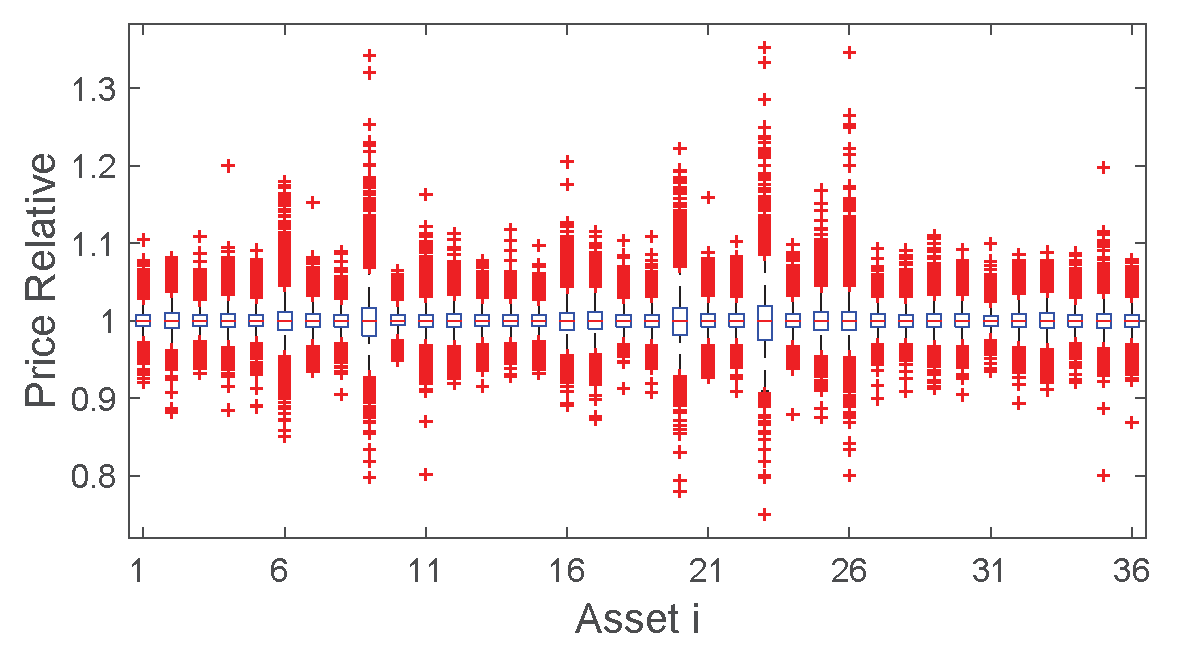
\includegraphics[width=0.49\textwidth]{./figure/boxplot_nyse-o.eps}}
	\subfloat[NYSE(N)]{
		\centering
		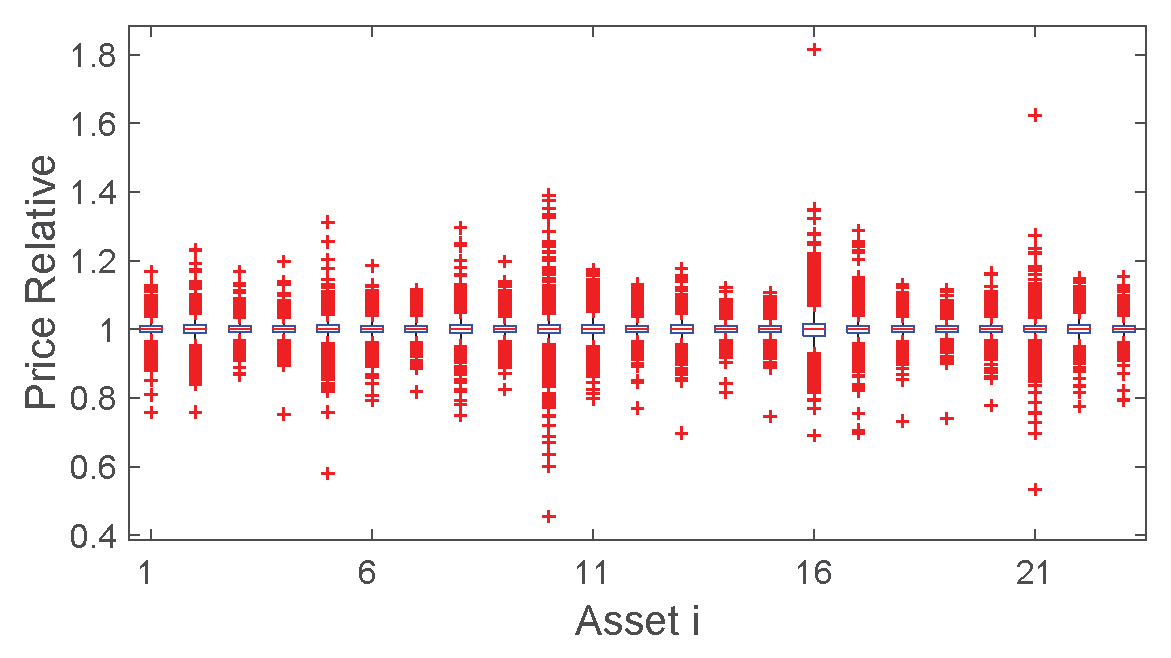
\includegraphics[width=0.49\textwidth]{./figure/boxplot_nyse-n.eps}}\\
		\subfloat[DJIA]{
		\centering
		\includegraphics[width=0.49\textwidth]{./figure/boxplot_djia.eps}}
	\subfloat[SP500]{
		\centering
		\includegraphics[width=0.49\textwidth]{./figure/boxplot_sp500.eps}}\\
	\subfloat[TSE]{
		\centering
		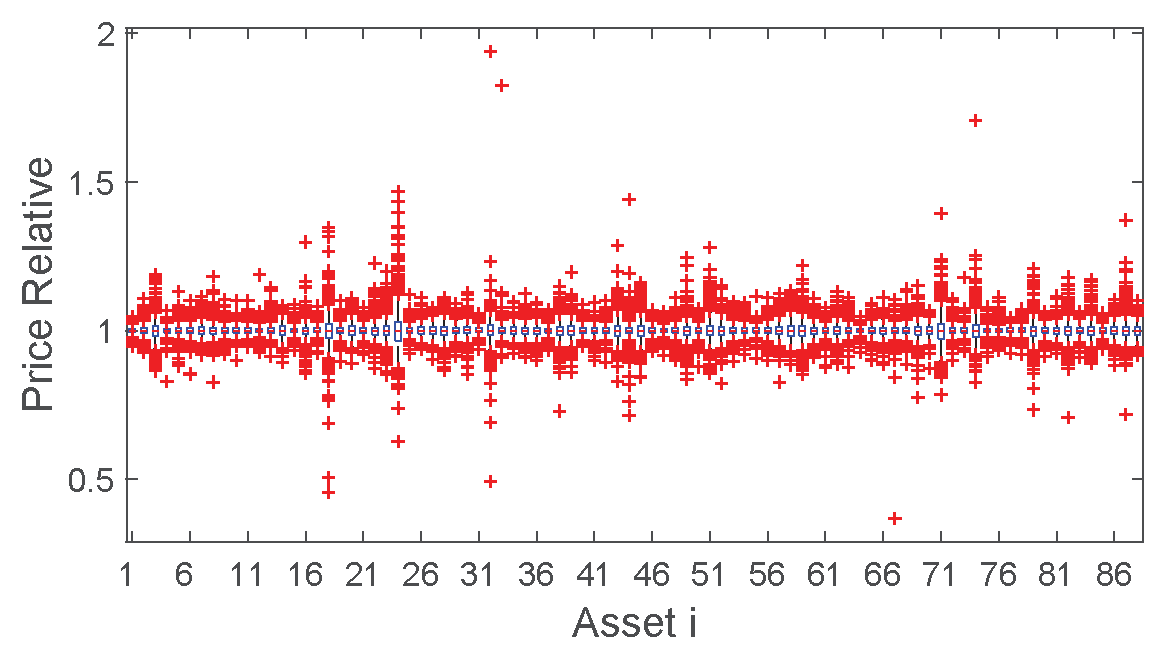
\includegraphics[width=1\textwidth]{./figure/boxplot_tse.eps}}
%		}
	\caption{Box plots of asset price relatives on $5$ benchmark data sets.}
	\label{fig:boxplotrela}
\end{figure*}


For comparison, $7$ state-of-the-art short-term PO systems are evaluated: ONS \citep{ONS}, CORN, Anticor, PAMR \citep{PAMR}, CWMR \citep{CWMR}, OLMAR and RMR, as well as $2$ trivial ones: Beststock and Market. The parameters for these systems are set by the defaults in their original papers and previous experiments \citep{olpssurvey,olpsjmlr,OLMAR,RMR2}: ONS: $\eta=0,\beta=1,\gamma=\frac{1}{8}$; CORN: $w = 5, P = 1, \rho = 0.1$; Anticor: $w=5$; PAMR and CWMR: $\epsilon=0.5$; OLMAR: $w=5, \epsilon=10$; RMR: $w=5,\epsilon=5$. The parameters for SSPO are set as: $w=5, \lambda=0.5, \gamma=0.01, \eta=0.005, \zeta=500$. Note that the window size $w=5$ is the same with all these systems, to be consistent.



Evaluation protocols mainly fall into $8$ indicators: 1. Cumulative wealth (CW): the main score to evaluate investing performance; 2. Mean Excess Return (MER) \citep{MR1}: the average excess performance of a system compared with the market; 3. $\alpha$ Factor \citep{portalpha0}: MER excluding the market risk; 4. Order statistics: the rank of a system return in all the asset returns; 5. Sharpe Ratio \citep{SHARPratio}: risk-adjusted average return; 6. Information Ratio \citep{inforatio2}: risk-adjusted MER; 7. Transaction costs; 8. Running times. Indicators 1$\sim$3 are investing performance measurements, Indicators 4$\sim$6 are risk metrics, and Indicators 7,8 evaluate the applicability to real-world financial environments. SSPO achieves state-of-the-art results in all these indicators.


\subsection{Parameter Setting}
\label{sec:paraset}
We first conduct experiments of the final cumulative wealth (CW) to empirically set the parameters for SSPO, which is similar to \citet{anticor,CORN,OLMAR,RMR,RMR2}. The final CW is the cumulative product of the actual increasing factors $\{\hat{\mathbf{b}}_{t}^\top\mathbf{x}_t\}_{t=1}^n$ with the initial wealth $S_0=1$. 

First, $w=5$ is a common window size in real-world stock trading, especially in short-term investment. It is also consistent with the compared state-of-the-art methods. Hence it is adopted for SSPO. Second, we fix $w=5$, $\gamma=0.01$, $\eta=0.005$, $\zeta=500$ and change $\lambda$ in $0.4\sim 0.65$. The results in Figure \ref{fig:parasetlbd} show that $\lambda=0.5$ leads to good performance in general and thus is set for SSPO. To better show the geometric scaling effect of the daily geometric increasing factor on the final CW, the power form is used to label the y-axis. The base is the daily geometric increasing factor while the exponent is the total number of trading days in the data set.

At each time, we change one parameter and fix other parameters, and the results are shown in Figure \ref{fig:paraseteta}, Figure \ref{fig:parasetgamma}, and Figure \ref{fig:parasetzeta}. They indicate that $\gamma=0.01$, $\eta=0.005$, and $\zeta=500$ are suitable parameters for SSPO.


\begin{figure*}[!htb]
	\centering
	\subfloat[NYSE(O)]{
		\centering
		\includegraphics[width=0.33\textwidth]{./figure/lambda_nyse_o.eps}}
	\subfloat[NYSE(N)]{
		\centering
		\includegraphics[width=0.33\textwidth]{./figure/lambda_nyse_n.eps}}
		\subfloat[DJIA]{
		\centering
		\includegraphics[width=0.33\textwidth]{./figure/lambda_djia.eps}}\\
	\subfloat[SP500]{
		\centering
		\includegraphics[width=0.33\textwidth]{./figure/lambda_sp500.eps}}
	\subfloat[TSE]{
		\centering
		\includegraphics[width=0.33\textwidth]{./figure/lambda_tse.eps}}
	\caption{Final cumulative wealths of SSPO with respect to $\lambda$ on $5$ benchmark data sets (fix $w=5$, $\gamma=0.01$, $\eta=0.005$, $\zeta=500$). The power form is used to label the y-axis to better show the geometric scaling effect of the daily geometric increasing factor on the final cumulative wealth. The base is the daily geometric increasing factor while the exponent is the total number of trading days in the data set.}
	\label{fig:parasetlbd}
\end{figure*}



\begin{figure*}[!htb]
	\centering
	\subfloat[NYSE(O)]{
		\centering
		\includegraphics[width=0.33\textwidth]{./figure/eta_nyse_o.eps}}
	\subfloat[NYSE(N)]{
		\centering
		\includegraphics[width=0.33\textwidth]{./figure/eta_nyse_n.eps}}
		\subfloat[DJIA]{
		\centering
		\includegraphics[width=0.33\textwidth]{./figure/eta_djia.eps}}\\
	\subfloat[SP500]{
		\centering
		\includegraphics[width=0.33\textwidth]{./figure/eta_sp500.eps}}
	\subfloat[TSE]{
		\centering
		\includegraphics[width=0.33\textwidth]{./figure/eta_tse.eps}}
	\caption{Final cumulative wealths of SSPO with respect to $\eta$ on $5$ benchmark data sets (fix $w=5$, $\gamma=0.01$, $\lambda=0.5$, $\zeta=500$).}
	\label{fig:paraseteta}
\end{figure*}



\begin{figure*}[!htb]
	\centering
	\subfloat[NYSE(O)]{
		\centering
		\includegraphics[width=0.33\textwidth]{./figure/gamma_nyse_o.eps}}
	\subfloat[NYSE(N)]{
		\centering
		\includegraphics[width=0.33\textwidth]{./figure/gamma_nyse_n.eps}}
		\subfloat[DJIA]{
		\centering
		\includegraphics[width=0.33\textwidth]{./figure/gamma_djia.eps}}\\
	\subfloat[SP500]{
		\centering
		\includegraphics[width=0.33\textwidth]{./figure/gamma_sp500.eps}}
	\subfloat[TSE]{
		\centering
		\includegraphics[width=0.33\textwidth]{./figure/gamma_tse.eps}}
	\caption{Final cumulative wealths of SSPO with respect to $\gamma$ on $5$ benchmark data sets (fix $w=5$, $\eta=0.005$, $\lambda=0.5$, $\zeta=500$).}
	\label{fig:parasetgamma}
\end{figure*}



\begin{figure*}[!htb]
	\centering
	\subfloat[NYSE(O)]{
		\centering
		\includegraphics[width=0.33\textwidth]{./figure/zeta_nyse_o.eps}}
	\subfloat[NYSE(N)]{
		\centering
		\includegraphics[width=0.33\textwidth]{./figure/zeta_nyse_n.eps}}
		\subfloat[DJIA]{
		\centering
		\includegraphics[width=0.33\textwidth]{./figure/zeta_djia.eps}}\\
	\subfloat[SP500]{
		\centering
		\includegraphics[width=0.33\textwidth]{./figure/zeta_sp500.eps}}
	\subfloat[TSE]{
		\centering
		\includegraphics[width=0.33\textwidth]{./figure/zeta_tse.eps}}
	\caption{Final cumulative wealths of SSPO with respect to $\zeta$ on $5$ benchmark data sets (fix $w=5$, $\eta=0.005$, $\lambda=0.5$, $\gamma=0.01$).}
	\label{fig:parasetzeta}
\end{figure*}



\subsection{Cumulative Wealth}
\label{sec:cumwealth}
We show the final CWs of different PO systems on $5$ benchmark data sets in Table \ref{tab:cmalpha}. The approximate power form is used to make an intuitive sense of the geometric scaling effect of the daily geometric increasing factor on the final CW. The base is the daily geometric increasing factor while the exponent is the total number of trading days in the data set. SSPO achieves the best performance on all the data sets against other state-of-the-art systems. For instance, SSPO achieves a much higher CW ($3.68$) than OLMAR ($2.54$) and RMR ($2.67$) on DJIA which is difficult to handle \citep{RMR2}. On NYSE(O), NYSE(N) and TSE, SSPO achieves CW$=1.06E{+}18$, $1.62E{+}9$ and $364.94$, respectively, which are much higher than OLMAR ($7.21E{+}16$, $4.14E{+}8$ and $58.51$) and RMR ($1.64E{+}17$, $3.25E{+}8$ and $181.34$). Therefore, SSPO is an efficient short-term PO system for diverse real-world stock markets. We also plot the CW evolution paths for different PO systems on DJIA in Figure \ref{fig:cwplots}. On most days, the SSPO plot is over other systems, and it climbs up significantly when there are good opportunities.

\begin{table}[!htb]
\centering
\scalebox{0.63}{
\begin{tabular}{|c|c|c|c|c|c|}
\hline
 &  {NYSE(O)}  & {NYSE(N)}  &{DJIA}  & {SP500}  &  {TSE}   \\
  \hline
  Market  &  $14.50\approx 1.00047^{5651}$     & $18.06\approx 1.00045^{6431}$     &  $0.76\approx 0.99947^{507}$     & $1.34\approx 1.00023^{1276}$     & $1.61\approx 1.00038^{1259}$  \\
  Beststock   & $54.14\approx 1.00071^{5651}$     & $83.51\approx 1.00069^{6431}$    &  $1.19\approx 1.00034^{507}$   &  $3.78\approx 1.00104^{1276}$   & $6.28\approx 1.00146^{1259}$   \\
    ONS   & $109.19\approx 1.00083^{5651}$  & $21.59\approx 1.00048^{6431}$  &  $1.53\approx 1.00084^{507}$  &  $3.34\approx 1.00095^{1276}$  & $1.62\approx 1.00038^{1259}$  \\
  CORN   & $8.09E{+}11\approx 1.00486^{5651}$  & $2.33E{+}5\approx 1.00192^{6431}$  &  $0.78\approx 0.99951^{507}$ &  $5.29\approx 1.00131^{1276}$  & $9.80\approx 1.000181^{1259}$    \\
  Anticor   & $2.04E{+}7\approx 1.00298^{5651}$   & $2.11E{+}5\approx 1.00191^{6431}$   &  $1.63\approx 1.00096^{507}$   &  $5.61\approx 1.00135^{1276}$   & $28.68\approx 1.00267^{1259}$  \\
  PAMR     & $5.14E{+}15\approx 1.00642^{5651}$   & $1.25E{+}6\approx 1.00219^{6431}$  &  $0.68\approx 0.99924^{507}$  &  $5.09\approx 1.00128^{1276}$   & $264.86\approx 1.00444^{1259}$   \\
  CWMR    & $6.49E{+}15\approx 1.00646^{5651}$   & $1.41E{+}6\approx 1.00220^{6431}$    &  $0.69\approx 0.99926^{507}$    &  $5.95\approx 1.00140^{1276}$    & $332.62\approx 1.00462^{1259}$ \\
  OLMAR   & $7.21E{+}16\approx 1.00689^{5651}$   & $4.14E{+}8\approx 1.00309^{6431}$  &  $2.54\approx 1.00184^{507}$    &  $15.94\approx 1.00217^{1276}$  & $58.51\approx 1.00324^{1259}$   \\
  RMR    & $1.64E{+}17\approx 1.00704^{5651}$   & $3.25E{+}8\approx 1.00305^{6431}$  &  $2.67\approx 1.00194^{507}$  &  $8.28\approx 1.00166^{1276}$  & $181.34\approx 1.00414^{1259}$   \\
\hline
  \textbf{SSPO}  & $\mathbf{1.06E{+}18\approx 1.00737^{5651}}$    & $\mathbf{1.62E{+}9\approx 1.00330^{6431}}$   &  $\mathbf{3.68\approx 1.00257^{507}}$   &  $\mathbf{16.97\approx 1.00222^{1276}}$  & $\mathbf{364.94\approx 1.00470^{1259}}$   \\
  \hline
\end{tabular}}
\caption{Final cumulative wealths of portfolio optimization systems on $5$ benchmark data sets. The approximate power form is used to make an intuitive sense of the geometric scaling effect of the daily geometric increasing factor on the final CW. The base is the daily geometric increasing factor while the exponent is the total number of trading days in the data set.}
\label{tab:cmalpha}
\end{table}


\begin{figure*}[!htb]
\centering
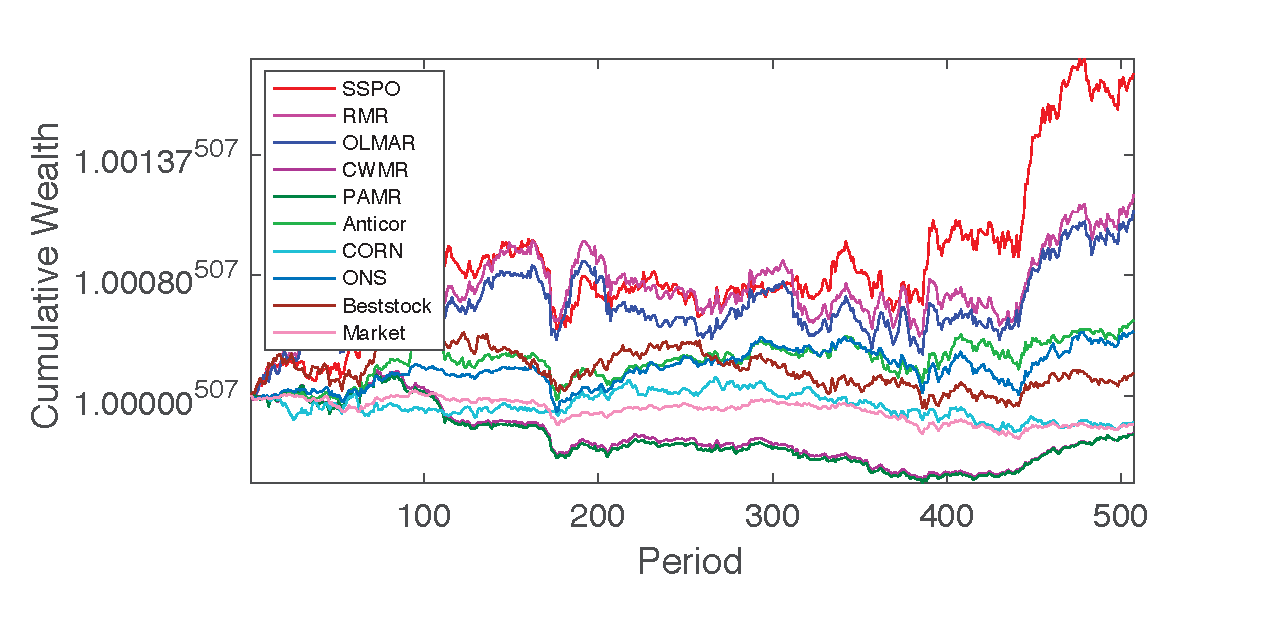
\includegraphics[width=\textwidth]{./figure/cw-djia.eps}\\
\caption{Cumulative wealth evolution paths of portfolio optimization systems on DJIA. The length of one period is one day.}
\label{fig:cwplots}
\end{figure*}





\subsection{Mean Excess Return}
\label{sec:MER}
At the end of each day, we want to know what proportion of total wealth gained or lost on this day. This concept can be represented by the term ``return'': $r_{t}=\hat{\mathbf{b}}_{t}^\top\mathbf{x}_t-1$. Mean Excess Return (MER) \citep{MR1} is the average daily excess return of a system compared with the market in the long run:
\begin{eqnarray}
\label{eqn:mer}
MER=\bar{r}_{s}-\bar{r}_{m}=\frac{1}{n}\sum_{t=1}^n ({r}_{s,t}-{r}_{m,t}),
\end{eqnarray}
where ${r}_{s,t}$ and ${r}_{m,t}$ are daily returns of a PO system and the market on the $t$-th day, respectively. It is more worthy of implementing a PO system with a higher MER. Even a small difference of MER leads to a large gap of CW in the long run, due to the geometric scaling effect.

We present the MERs for different PO systems in Table \ref{tab:mer}. SSPO outperforms other state-of-the-art systems on all the data sets. For instance, the MERs of SSPO ($0.0036$ and $0.0060$) are much higher than those of OLMAR ($0.0028$ and $0.0045$) and RMR ($0.0029$ and $0.0053$) on DJIA and TSE, respectively. This is the reason why SSPO outperforms other systems in cumulative wealth in the long run.

\begin{table*}[!htb]
\centering
\footnotesize
\begin{tabular}{|c|c|c|c|c|c|}
\hline
 System & {NYSE(O)}  &  {NYSE(N)}  &{DJIA}  & {SP500}  &  {TSE}   \\
  \hline
  Beststock   & $0.0003$  &  $0.0003$   & $0.0011$   & $0.0012$   & $0.0016$   \\
    ONS   & $0.0004$  & $0.0003$   & $0.0015$   & $0.0007$   & $0.0002$  \\
  CORN     & $0.0049$    & $0.0017$  & $0.0002$  & $0.0014$  & $0.0020$  \\
  Anticor     & $0.0026$   & $0.0016$   & $0.0016$  & $0.0013$  & $0.0027$  \\
  PAMR     & $0.0064$    & $0.0021$  & $0.0001$  & $0.0014$   & $0.0050$ \\
  CWMR     & $0.0064$    & $0.0022$  & $0.0001$  & $0.0015$   & $0.0053$ \\
  OLMAR     & $0.0070$    & $0.0032$  & $0.0028$  & $0.0024$  & $0.0045$  \\
  RMR    & $0.0071$   & $0.0032$  & $0.0029$ & $0.0019$  & $0.0053$ \\
\hline
  \textbf{SSPO}  & $\mathbf{0.0076}$  & $\mathbf{0.0035}$  &  $\mathbf{0.0036}$  &  $\mathbf{0.0025}$  & $\mathbf{0.0060}$  \\
  \hline
\end{tabular}
\normalsize
\caption{Mean excess returns of portfolio optimization systems on $5$ benchmark data sets.}
\label{tab:mer}
\end{table*}





\subsection{$\alpha$ Factor}
\label{sec:alphafactor}
According to the Capital Asset Pricing Model (CAPM) \citep{CAPM}, the expected return of a system can be decomposed into $2$ parts: the market return component, and the intrinsic excess return usually called the $\alpha$ Factor in the finance industry \citep{portalpha0}. The former is determined by the market environment, which cannot be improved by any active investing strategy or PO system, while the latter can be improved by a good PO system. The $\alpha$ Factor can be represented as follows:
\begin{eqnarray}
\label{eqn:alphafactor}
E({r}_{s})&=&\beta E({r}_{m})+\alpha,\\
\label{eqn:betaestimate}
\hat{\beta}&=&\frac{\hat{c}({r}_{s},{r}_{m})}{\hat{\sigma}^2({r}_{m})},\quad \hat{\alpha}=\bar{r}_{s}-\hat{\beta}\bar{r}_{m},
\end{eqnarray}
where $E(\cdot)$ denotes the mathematical expectation, $\hat{c}(\cdot,\cdot)$ and $\hat{\sigma}(\cdot)$ are the sample covariance and the sample standard deviation (STD) computed on $n$ trading days, respectively. In finance, STD is a common tool to measure risk (volatility).

The $\alpha$ Factors of different PO systems are given in Table \ref{tab:alphafactor}. SSPO outperforms other PO systems on all the data sets, indicating that SSPO achieves high intrinsic excess returns despite the market volatility. Particularly on DJIA data set which is difficult to handle, SSPO achieves $\alpha=0.0037$, which is much higher than OLMAR ($0.0029$) and RMR ($0.0030$).

In the real-world portfolio management, it is common to perform a right-tailed t-test to see whether $\alpha$ is significantly $>0$. If so, it indicates that the good performance of the system is not due to luck \citep{activepm,OLMAR,RMR,RMR2}. According to the results in Table \ref{tab:alphafactor}, SSPO achieves significantly better performance than the market at a high confidence level of $99\%$ (with all $p$-values $<0.01$).



\begin{table*}[!htb]
\centering
\scalebox{0.76}{
\begin{tabular}{|c|c|c|c|c|c|c|c|c|c|c|}
\hline
 \multirow{2}{*}{System} &  \multicolumn{2}{|c|}{NYSE(O)}  &  \multicolumn{2}{|c|}{NYSE(N)}  &\multicolumn{2}{|c|}{DJIA}  & \multicolumn{2}{|c|}{SP500}  &  \multicolumn{2}{|c|}{TSE}   \\
 \cline{2-11}
 & $\alpha$ &  p-Value  & $\alpha$ &  p-Value  & $\alpha$ & p-Value   & $\alpha$ &  p-Value & $\alpha$ & p-Value\\
  \hline
  Beststock   & $0.0003$  &  $0.0195$  & $0.0004$   &  $0.0176$ & $0.0012$   &  $0.0838$ & $0.0011$   &  $0.0593$ & $0.0014$   &  $0.0606$ \\
    ONS   & $0.0005$  &  $<0.0001$  & $0.0003$   &  $0.1257$ & $0.0016$   &  $<0.0001$ & $0.0008$   &  $0.0040$ & $0.0002$   &  $0.3514$ \\
  CORN     & $0.0048$   &  $<0.0001$   & $0.0016$   & $<0.0001$ & $0.0002$   &  $0.4077$ & $0.0013$   &  $0.0190$ & $0.0018$   &  $0.0278$ \\
  Anticor     & $0.0026$   &  $<0.0001$   & $0.0016$   &  $<0.0001$ & $0.0017$  &  $0.0010$  & $0.0012$   &  $0.0021$ & $0.0025$   &  $<0.0001$ \\
  PAMR     & $0.0063$   &  $<0.0001$   & $0.0021$   &   $<0.0001$ & $0.0002$  &  $0.4275$  & $0.0013$   &   $0.0259$ & $0.0048$   &  $<0.0001$ \\
  CWMR     & $0.0063$   &  $<0.0001$   & $0.0021$   &  $<0.0001$ & $0.0002$  &  $0.4168$  & $0.0014$   &  $0.0170$   & $0.0051$   & $<0.0001$ \\
  OLMAR     & $0.0069$   &  $<0.0001$   & $0.0031$   &   $<0.0001$ & $0.0029$   &  $0.0065$ & $0.0023$   &  $0.0017$ & $0.0042$   &  $0.0050$ \\
  RMR    & $0.0070$   &  $<0.0001$   & $0.0031$   &  $<0.0001$ & $0.0030$   &  $0.0054$ & $0.0018$   &   $0.0102$ & $0.0051$   &  $<0.0001$ \\
\hline
  \textbf{SSPO}  & $\mathbf{0.0074}$   &  $<0.0001$  & $\mathbf{0.0034}$   & $<0.0001$  &  $\mathbf{0.0037}$   &  $0.0009$ &  $\mathbf{0.0024}$   &  $0.0019$ & $\mathbf{0.0058}$   &  $<0.0001$  \\
  \hline
\end{tabular}
}
\caption{$\alpha$ factors (with p-values of t-tests) of portfolio optimization systems on $5$ benchmark data sets.}
\label{tab:alphafactor}
\end{table*}




\subsection{Order Statistics}
\label{sec:orderstat}
One may worry about that a PO system just simply selects the lucky assets with the highest growth. To check this point, we can compare the system return $r_{s,t}=\hat{\mathbf{b}}_{t}^\top\mathbf{x}_t-1$ with all the asset returns $r_{t}^{(i)}=\mathbf{x}_t^{(i)}-1$, $i=1,\cdots,d$ ($d$ is the number of assets in a data set). By sorting the $(d+1)$ returns $\{r_{s,t}\}\bigcup\{r_{t}^{(i)}\}_{i=1}^d$ in the descending order, we can obtain the rank of $r_{s,t}$. If a PO system always chooses the lucky assets, then $r_{s,t}$ will always rank very high in the investment.

We give a summary description of the rank of $r_{s,t}$ in the whole investment ($n$ days) on each data set for different PO systems, shown in Figure \ref{fig:boxplotrank} and Table \ref{tab:rank}. It can be seen that the ranks for SSPO cover a wide range instead of concentrating on the highest ranks. Besides, the mean rank and the median rank of SSPO are close to the middle rank $(d+1)/2$ on each data set, indicating that SSPO is at the average return level of all the asset returns. Furthermore, the rank results of SSPO are similar to other state-of-the-art short-term PO systems, which means that SSPO has a similar return level to the related systems. To summarize, SSPO does not simply select the lucky assets with the highest growth and its returns are credible. Note that this rank test is different from the rank-dependent portfolio \citep{stoport} that takes the rank information as prior knowledge and exploits it to formulate PO models.

\begin{figure*}[!htb]
	\centering
	\subfloat[NYSE(O)]{
		\centering
		\includegraphics[width=0.324\textwidth]{./figure/rank_nyse_o.eps}}
	\subfloat[NYSE(N)]{
		\centering
		\includegraphics[width=0.324\textwidth]{./figure/rank_nyse_n.eps}}
		\subfloat[DJIA]{
		\centering
		\includegraphics[width=0.324\textwidth]{./figure/rank_djia.eps}}\\
	\subfloat[SP500]{
		\centering
		\includegraphics[width=0.324\textwidth]{./figure/rank_sp500.eps}}
	\subfloat[TSE]{
		\centering
		\includegraphics[width=0.324\textwidth]{./figure/rank_tse.eps}}
	\caption{Box plots of the ranks for the system returns $r_{s,t}$ on $5$ benchmark data sets. The ranks for SSPO cover a wide range instead of concentrating on the highest ranks.}
	\label{fig:boxplotrank}
\end{figure*}

\begin{table*}[!htb]
\centering
\footnotesize
\begin{tabular}{|c|c|c|c|c|c|c|c|c|c|c|}
\hline
 \multirow{2}{*}{System} &  \multicolumn{2}{|c|}{NYSE(O): $37$}  &  \multicolumn{2}{|c|}{NYSE(N): $24$}  &\multicolumn{2}{|c|}{DJIA: $31$}  & \multicolumn{2}{|c|}{SP500: $26$}  &  \multicolumn{2}{|c|}{TSE: $89$}   \\
 \cline{2-11}
 & Median & Mean   & Median & Mean   & Median & Mean   & Median & Mean  & Median & Mean\\
  \hline
  Market   & $19$  &  $18.63$  & $12$   &  $12.25$ & $16$   & $16.12$  & $13$   & $13.34$  & $43$   &  $42.88$ \\
  Beststock   & $19$  &  $19.34$  & $13$   &  $12.76$ & $16$   &  $16.32$ & $14$   &  $14.05$ & $52$   &  $47.09$ \\
    ONS   & $19$  &  $18.56$  & $12$   &  $12.42$ & $15$   &  $15.35$ & $13$   &  $13.01$ & $45$   &  $44.83$ \\
  CORN     & $18$   &  $18.08$   & $12$   &  $12.10$ & $16$   &  $16.04$ & $13$   &  $13.26$ & $46$   &  $44.87$ \\
  Anticor     & $17$   &  $17.25$   & $12$   &  $11.72$ & $15$  &  $15.32$  & $13$   &  $12.98$ & $39$   &  $41.77$ \\
  PAMR     & $16$   &  $17.27$   & $12$   &  $12.22$ & $15$  &  $16.05$  & $13$   &  $13.22$ & $35$   &  $40.11$ \\
  CWMR     & $16$   &  $17.22$   & $12$   &  $12.19$ & $16$  &  $16.09$  & $13$   &  $13.18$ & $35$   &  $40.01$ \\
  OLMAR     & $17$   &  $17.56$   & $12$   &  $12.26$ & $15$   &  $15.45$ & $12$   &  $13.31$ & $43$   &  $43.12$ \\
  RMR    & $16$   &  $17.40$   & $12$   &  $12.26$ & $15$   &  $15.34$ & $13$   &  $13.40$ & $40$   &  $42.18$ \\
\hline
  \textbf{SSPO}  & $17$   &  $17.71$  & $12$   &  $12.25$  &  $15$   &  $15.25$ &  $12$   &  $13.33$ & $44$   &  $43.03$  \\
  \hline
\end{tabular}
\normalsize
\caption{Medians and means of the ranks for the system returns $r_{s,t}$ on $5$ benchmark data sets. The value of $(d+1)$ is also given behind each data set name. The mean rank and the median rank of SSPO are close to the middle rank $(d+1)/2$ on each data set, which indicates that SSPO does not simply select the lucky assets with the highest growth.}
\label{tab:rank}
\end{table*}
\newpage



\subsection{Sharpe Ratio}
\label{sec:sharperatio}
In general, when an investor pursues high return, he/she should be ready to undertake high risk. Thus he/she has to balance between return and risk all the time. Sharpe Ratio (SR) \citep{SHARPratio} is such a measurement to meet this demand based on CAPM:
\begin{eqnarray}
\label{eqn:sharperatio}
SR=\frac{\bar{r}_{s}-{r}_{f}}{\hat{\sigma}({r}_{s})},
\end{eqnarray}
where ${r}_{f}$ is the daily return of some risk-free asset, which is not considered in this paper. Hence we set ${r}_{f}=0$ to make SR a daily risk-adjusted return.

We compute and present the daily SRs of different PO systems in Table \ref{tab:srir}. SSPO achieves the highest SR on NYSE(N) and DJIA, and is close to the best system on other data sets. Besides, SSPO is competitive to OLMAR and RMR. For example, SSPO achieves $SR=0.0791$ on SP500 compared with RMR ($0.0659$), and achieves $SR=0.1054$ on TSE compared with OLMAR ($0.0820$). It indicates that SSPO has a good ability in balancing between return and risk on the premise of good investing achievement with high CWs.



\begin{table*}[!htb]
\centering
\scalebox{0.81}{
\begin{tabular}{|c|c|c|c|c|c|c|c|c|c|c|}
\hline
 \multirow{2}{*}{System} &  \multicolumn{2}{|c|}{NYSE(O)}  &  \multicolumn{2}{|c|}{NYSE(N)}  &\multicolumn{2}{|c|}{DJIA}  & \multicolumn{2}{|c|}{SP500}  &  \multicolumn{2}{|c|}{TSE}   \\
 \cline{2-11}
 & SR & IR   & SR & IR   & SR & IR   & SR & IR  & SR & IR\\
  \hline
  Market   & $0.0549$  &  Null  & $0.0458$   &  Null & $-0.0273$   & Null  & $0.0224$   & Null  & $0.0491$   &  Null \\
  Beststock   & $0.0536$  &  $0.0241$  & $0.0472$   &  $0.0225$ & $0.0253$   &  $0.0560$ & $0.0485$   &  $0.0468$ & $0.0579$   &  $0.0490$ \\
    ONS   & $0.0789$  &  $0.0424$  & $0.0313$   &  $0.0129$ & $0.0504$   &  $\mathbf{0.1574}$ & $0.0701$   &  $0.0582$ & $0.0281$   &  $0.0093$ \\
  CORN     & $0.1635$   &  $0.1570$   & $0.0968$   &  $0.0859$ & $-0.0097$   &  $0.0108$ & $0.0581$   &  $0.0618$ & $0.0675$   &  $0.0595$ \\
  Anticor     & $0.1720$   &  $0.1743$   & $0.0973$   &  $0.0899$ & $0.0535$  &  $0.1255$  & $0.0682$   &  $0.0834$ & $0.1061$   &  $0.0993$ \\
  PAMR     & $0.2149$   &  $0.2121$   & $0.0864$   &  $0.0763$ & $-0.0115$  &  $0.0036$  & $0.0568$   &  $0.0573$ & $\mathbf{0.1182}$   &  $\mathbf{0.1131}$ \\
  CWMR     & $\mathbf{0.2169}$   &  $\mathbf{0.2143}$   & $0.0858$   &  $0.0758$ & $-0.0106$  &  $0.0047$  & $0.0606$   &  $0.0623$ & $0.1179$   &  $0.1129$ \\
  OLMAR     & $0.2102$   &  $0.2071$   & $0.1038$   &  $0.0958$ & $0.0731$   &  $0.1058$ & $\mathbf{0.0806}$   &  $\mathbf{0.0848}$ & $0.0820$   &  $0.0769$ \\
  RMR    & $0.2153$   &  $0.2123$   & $0.1033$   &  $0.0953$ & $0.0763$   &  $0.1092$ & $0.0659$   &  $0.0678$ & $0.0981$   &  $0.0932$ \\
\hline
  \textbf{SSPO}  & $\mathbf{0.2073}$   &  $\mathbf{0.2041}$  & $\mathbf{0.1060}$   &  $\mathbf{0.0979}$  &  $\mathbf{0.0919}$   &  $\mathbf{0.1304}$ &  $\mathbf{0.0791}$   &  $\mathbf{0.0840}$ & $\mathbf{0.1054}$   &  $\mathbf{0.1009}$  \\
  \hline
\end{tabular}
}
\caption{Daily Sharpe Ratios (SR) and daily Information Ratios (IR) of portfolio optimization systems on $5$ benchmark data sets.}
\label{tab:srir}
\end{table*}



\subsection{Information Ratio}
\label{sec:inforatio}
Different from SR, Information Ratio (IR) \citep{inforatio2} directly measures the daily risk-adjusted excess return of a system compared with the market, which can be seen as a combination of MER and SR. It is also worth reference for the concern with risk.
\begin{eqnarray}
\label{eqn:inforatio}
IR=\frac{(\bar{r}_{s}-\bar{r}_{m})}{\hat{\sigma}({r}_{s}-{r}_{m})}.
\end{eqnarray}

We compute the daily IRs of different PO systems in Table \ref{tab:srir}. SSPO achieves the highest IR on NYSE(N) and is close to the best system on other data sets. Moreover, SSPO is competitive to OLMAR and RMR. For example,  SSPO achieves $IR=0.0840, 0.1009$ on SP500 and TSE, respectively, while RMR achieves $IR=0.0678$ on SP500 and OLMAR achieves $IR=0.0769$ on TSE. It shows the robustness of SSPO to risk on the premise of good investing performance.



\subsection{Transaction Costs}
\label{sec:tc}
In practice, transaction cost is an important issue in PO. Suppose we have to pay at a transaction cost rate $\nu\in(0,1)$ to update the portfolio. Then according to the proportional transaction cost model \citep{UPtc,OLMAR,RMR2}, the cumulative wealth at the beginning of the $t$-th day is
\begin{eqnarray}
  S_n^{\nu} &=& S_0\prod_{t=1}^{n}[(\hat{\mathbf{b}}_t^\top\mathbf{x}_t)\cdot
  (1-\frac{\nu}{2}\sum_{i=1}^{d}|\hat{\mathbf{b}}_t^{(i)}-\tilde{\mathbf{b}}_{t-1}^{(i)}|)], \\
  \tilde{\mathbf{b}}_{t-1}^{(i)} &=& \frac{\hat{\mathbf{b}}_{t-1}^{(i)}\cdot\mathbf{x}_{t-1}^{(i)}}{\hat{\mathbf{b}}_{t-1}^\top\mathbf{x}_{t-1}},
\end{eqnarray}
where $\tilde{\mathbf{b}}_{t-1}^{(i)}$ denotes the adjusted portfolio of Asset $i$ at the end of the $(t-1)$-th day and $\tilde{\mathbf{b}}_{0}$ is set as $[0,\cdots,0]^\top$. $\frac{\nu}{2}\sum_{i=1}^{d}|\hat{\mathbf{b}}_t^{(i)}-\tilde{\mathbf{b}}_{t-1}^{(i)}|$ is the proportional transaction cost when we change the adjusted portfolio $\tilde{\mathbf{b}}_{t-1}$ to the next portfolio $\hat{\mathbf{b}}_{t}$.

To test the effectiveness of SSPO with consideration of transaction cost, we conduct experiments of cumulative wealth with $\nu=0\sim0.5\%$, where $\nu=0.5\%$ is a rather high cost rate for stock transactions. The results shown in Figure \ref{fig:tc} indicate that SSPO outperforms the two state-of-the-art systems OLMAR and RMR on all the data sets and thus it is applicable to real-world financial environments.

\begin{figure*}[!htb]
\centering
\subfloat[NYSE(O)]{
\centering
\includegraphics[width=0.33\textwidth]{./figure/tc_nyse_o.eps}}
\subfloat[NYSE(N)]{
\centering
\includegraphics[width=0.33\textwidth]{./figure/tc_nyse_n.eps}}
\subfloat[DJIA]{
\centering
\includegraphics[width=0.33\textwidth]{./figure/tc_djia.eps}}\\
\subfloat[SP500]{
\centering
\includegraphics[width=0.33\textwidth]{./figure/tc_sp500.eps}}
\subfloat[TSE]{
\centering
\includegraphics[width=0.33\textwidth]{./figure/tc_tse.eps}}
\caption{Cumulative wealths of portfolio optimization systems with respect to the transaction cost rate $\nu$ on $5$ benchmark data sets.}
\label{fig:tc}
\end{figure*}



\subsection{Running Times}
\label{sec:comcost}
We use a computer with an AMD A10-7800 CPU and an 8GB DDR3 1600MHz memory card to run SSPO in the experiments, which shows that it is sufficiently fast for large-scale and time-limited trading environments such as High-Frequency Trading (HFT) \citep{HFT}. The average running times (in seconds) of SSPO for one trade on different data sets are: NYSE(O) ($0.0576$s), NYSE(N) ($0.0450$s), DJIA ($0.0455$s), SP500 ($0.0449$s), and TSE ($0.1190$s). Hence SSPO has good computational efficiency besides significant investing advantage.











\section{Conclusions}
\label{sec:conclusion}
We present a novel short-term sparse portfolio optimization (SSPO) system to concentrate wealth on a few assets with good increasing potential according to some empirical financial principles. Few short-term PO systems construct sparse portfolios, and most existing sparsity systems are either lazy updates or for the long-term PO. These problems motivate the design of SSPO. We further propose an ADMM algorithm for SSPO, and prove that its augmented Lagrangian has a saddle point. This is the foundation of the iterative formulae of ADMM but is seldom addressed before. 

We conduct extensive experiments on $5$ benchmark data sets with diverse real-world stock data, which shows that SSPO outperforms other state-of-the-art short-term PO systems with all the investing performance measurements (cumulative wealth, mean excess return and $\alpha$ Factor) on all the benchmark data sets. The order statistics of the SSPO returns also indicate that SSPO does not simply select the lucky assets with the highest growth and its returns are credible. SSPO is also competitive to other systems on the risk metrics SR and IR, and shows robustness in balancing between return and risk. Furthermore, SSPO can withstand reasonable transaction costs and runs fast, thus it is applicable to real-world financial environments including High-Frequency Trading. Therefore, SSPO is an effective and robust system that is worth further investigations. In the future, we will continue to establish more complex SSPO systems, so as to improve the investing performance and the robustness to risk.









% Acknowledgements should go at the end, before appendices and references

\acks{This work is supported in part by the National Natural Science Foundation of China under Grants 61703182, 61603152, 61602211, in part by the Talent Introduction Foundation of Jinan University under Grants 88016653, 88016534, in part by the Fundamental Research Funds for the Central Universities under Grants 21617347, 21617404, in part by the Fundamental Research Funds for the Center for Mathematical Finance in Guangdong Province under Grant 50411628, in part by the Science and Technology Program of Guangzhou, China under Grant 201707010259, and in part by the Guangxi Key Laboratory of Trusted Software (No. kx201606). }

% Manual newpage inserted to improve layout of sample file - not
% needed in general before appendices/bibliography.

%\newpage

%\appendix
%\section*{Appendix A.}



\vskip 0.2in

\bibliography{qrref}
%\bibliographystyle{natbib}

\end{document}
